% Options for packages loaded elsewhere
\PassOptionsToPackage{unicode}{hyperref}
\PassOptionsToPackage{hyphens}{url}
\PassOptionsToPackage{dvipsnames,svgnames,x11names}{xcolor}
%
\documentclass[
  letterpaper,
  DIV=11,
  numbers=noendperiod]{scrreprt}

\usepackage{amsmath,amssymb}
\usepackage{iftex}
\ifPDFTeX
  \usepackage[T1]{fontenc}
  \usepackage[utf8]{inputenc}
  \usepackage{textcomp} % provide euro and other symbols
\else % if luatex or xetex
  \usepackage{unicode-math}
  \defaultfontfeatures{Scale=MatchLowercase}
  \defaultfontfeatures[\rmfamily]{Ligatures=TeX,Scale=1}
\fi
\usepackage{lmodern}
\ifPDFTeX\else  
    % xetex/luatex font selection
\fi
% Use upquote if available, for straight quotes in verbatim environments
\IfFileExists{upquote.sty}{\usepackage{upquote}}{}
\IfFileExists{microtype.sty}{% use microtype if available
  \usepackage[]{microtype}
  \UseMicrotypeSet[protrusion]{basicmath} % disable protrusion for tt fonts
}{}
\makeatletter
\@ifundefined{KOMAClassName}{% if non-KOMA class
  \IfFileExists{parskip.sty}{%
    \usepackage{parskip}
  }{% else
    \setlength{\parindent}{0pt}
    \setlength{\parskip}{6pt plus 2pt minus 1pt}}
}{% if KOMA class
  \KOMAoptions{parskip=half}}
\makeatother
\usepackage{xcolor}
\setlength{\emergencystretch}{3em} % prevent overfull lines
\setcounter{secnumdepth}{5}
% Make \paragraph and \subparagraph free-standing
\ifx\paragraph\undefined\else
  \let\oldparagraph\paragraph
  \renewcommand{\paragraph}[1]{\oldparagraph{#1}\mbox{}}
\fi
\ifx\subparagraph\undefined\else
  \let\oldsubparagraph\subparagraph
  \renewcommand{\subparagraph}[1]{\oldsubparagraph{#1}\mbox{}}
\fi

\usepackage{color}
\usepackage{fancyvrb}
\newcommand{\VerbBar}{|}
\newcommand{\VERB}{\Verb[commandchars=\\\{\}]}
\DefineVerbatimEnvironment{Highlighting}{Verbatim}{commandchars=\\\{\}}
% Add ',fontsize=\small' for more characters per line
\usepackage{framed}
\definecolor{shadecolor}{RGB}{241,243,245}
\newenvironment{Shaded}{\begin{snugshade}}{\end{snugshade}}
\newcommand{\AlertTok}[1]{\textcolor[rgb]{0.68,0.00,0.00}{#1}}
\newcommand{\AnnotationTok}[1]{\textcolor[rgb]{0.37,0.37,0.37}{#1}}
\newcommand{\AttributeTok}[1]{\textcolor[rgb]{0.40,0.45,0.13}{#1}}
\newcommand{\BaseNTok}[1]{\textcolor[rgb]{0.68,0.00,0.00}{#1}}
\newcommand{\BuiltInTok}[1]{\textcolor[rgb]{0.00,0.23,0.31}{#1}}
\newcommand{\CharTok}[1]{\textcolor[rgb]{0.13,0.47,0.30}{#1}}
\newcommand{\CommentTok}[1]{\textcolor[rgb]{0.37,0.37,0.37}{#1}}
\newcommand{\CommentVarTok}[1]{\textcolor[rgb]{0.37,0.37,0.37}{\textit{#1}}}
\newcommand{\ConstantTok}[1]{\textcolor[rgb]{0.56,0.35,0.01}{#1}}
\newcommand{\ControlFlowTok}[1]{\textcolor[rgb]{0.00,0.23,0.31}{#1}}
\newcommand{\DataTypeTok}[1]{\textcolor[rgb]{0.68,0.00,0.00}{#1}}
\newcommand{\DecValTok}[1]{\textcolor[rgb]{0.68,0.00,0.00}{#1}}
\newcommand{\DocumentationTok}[1]{\textcolor[rgb]{0.37,0.37,0.37}{\textit{#1}}}
\newcommand{\ErrorTok}[1]{\textcolor[rgb]{0.68,0.00,0.00}{#1}}
\newcommand{\ExtensionTok}[1]{\textcolor[rgb]{0.00,0.23,0.31}{#1}}
\newcommand{\FloatTok}[1]{\textcolor[rgb]{0.68,0.00,0.00}{#1}}
\newcommand{\FunctionTok}[1]{\textcolor[rgb]{0.28,0.35,0.67}{#1}}
\newcommand{\ImportTok}[1]{\textcolor[rgb]{0.00,0.46,0.62}{#1}}
\newcommand{\InformationTok}[1]{\textcolor[rgb]{0.37,0.37,0.37}{#1}}
\newcommand{\KeywordTok}[1]{\textcolor[rgb]{0.00,0.23,0.31}{#1}}
\newcommand{\NormalTok}[1]{\textcolor[rgb]{0.00,0.23,0.31}{#1}}
\newcommand{\OperatorTok}[1]{\textcolor[rgb]{0.37,0.37,0.37}{#1}}
\newcommand{\OtherTok}[1]{\textcolor[rgb]{0.00,0.23,0.31}{#1}}
\newcommand{\PreprocessorTok}[1]{\textcolor[rgb]{0.68,0.00,0.00}{#1}}
\newcommand{\RegionMarkerTok}[1]{\textcolor[rgb]{0.00,0.23,0.31}{#1}}
\newcommand{\SpecialCharTok}[1]{\textcolor[rgb]{0.37,0.37,0.37}{#1}}
\newcommand{\SpecialStringTok}[1]{\textcolor[rgb]{0.13,0.47,0.30}{#1}}
\newcommand{\StringTok}[1]{\textcolor[rgb]{0.13,0.47,0.30}{#1}}
\newcommand{\VariableTok}[1]{\textcolor[rgb]{0.07,0.07,0.07}{#1}}
\newcommand{\VerbatimStringTok}[1]{\textcolor[rgb]{0.13,0.47,0.30}{#1}}
\newcommand{\WarningTok}[1]{\textcolor[rgb]{0.37,0.37,0.37}{\textit{#1}}}

\providecommand{\tightlist}{%
  \setlength{\itemsep}{0pt}\setlength{\parskip}{0pt}}\usepackage{longtable,booktabs,array}
\usepackage{calc} % for calculating minipage widths
% Correct order of tables after \paragraph or \subparagraph
\usepackage{etoolbox}
\makeatletter
\patchcmd\longtable{\par}{\if@noskipsec\mbox{}\fi\par}{}{}
\makeatother
% Allow footnotes in longtable head/foot
\IfFileExists{footnotehyper.sty}{\usepackage{footnotehyper}}{\usepackage{footnote}}
\makesavenoteenv{longtable}
\usepackage{graphicx}
\makeatletter
\def\maxwidth{\ifdim\Gin@nat@width>\linewidth\linewidth\else\Gin@nat@width\fi}
\def\maxheight{\ifdim\Gin@nat@height>\textheight\textheight\else\Gin@nat@height\fi}
\makeatother
% Scale images if necessary, so that they will not overflow the page
% margins by default, and it is still possible to overwrite the defaults
% using explicit options in \includegraphics[width, height, ...]{}
\setkeys{Gin}{width=\maxwidth,height=\maxheight,keepaspectratio}
% Set default figure placement to htbp
\makeatletter
\def\fps@figure{htbp}
\makeatother

\usepackage{fontspec}
\usepackage{multirow}
\usepackage{multicol}
\usepackage{colortbl}
\usepackage{hhline}
\newlength\Oldarrayrulewidth
\newlength\Oldtabcolsep
\usepackage{longtable}
\usepackage{array}
\usepackage{hyperref}
\usepackage{float}
\usepackage{wrapfig}
\KOMAoption{captions}{tableheading}
\makeatletter
\@ifpackageloaded{tcolorbox}{}{\usepackage[skins,breakable]{tcolorbox}}
\@ifpackageloaded{fontawesome5}{}{\usepackage{fontawesome5}}
\definecolor{quarto-callout-color}{HTML}{909090}
\definecolor{quarto-callout-note-color}{HTML}{0758E5}
\definecolor{quarto-callout-important-color}{HTML}{CC1914}
\definecolor{quarto-callout-warning-color}{HTML}{EB9113}
\definecolor{quarto-callout-tip-color}{HTML}{00A047}
\definecolor{quarto-callout-caution-color}{HTML}{FC5300}
\definecolor{quarto-callout-color-frame}{HTML}{acacac}
\definecolor{quarto-callout-note-color-frame}{HTML}{4582ec}
\definecolor{quarto-callout-important-color-frame}{HTML}{d9534f}
\definecolor{quarto-callout-warning-color-frame}{HTML}{f0ad4e}
\definecolor{quarto-callout-tip-color-frame}{HTML}{02b875}
\definecolor{quarto-callout-caution-color-frame}{HTML}{fd7e14}
\makeatother
\makeatletter
\@ifpackageloaded{bookmark}{}{\usepackage{bookmark}}
\makeatother
\makeatletter
\@ifpackageloaded{caption}{}{\usepackage{caption}}
\AtBeginDocument{%
\ifdefined\contentsname
  \renewcommand*\contentsname{Table of contents}
\else
  \newcommand\contentsname{Table of contents}
\fi
\ifdefined\listfigurename
  \renewcommand*\listfigurename{List of Figures}
\else
  \newcommand\listfigurename{List of Figures}
\fi
\ifdefined\listtablename
  \renewcommand*\listtablename{List of Tables}
\else
  \newcommand\listtablename{List of Tables}
\fi
\ifdefined\figurename
  \renewcommand*\figurename{Figure}
\else
  \newcommand\figurename{Figure}
\fi
\ifdefined\tablename
  \renewcommand*\tablename{Table}
\else
  \newcommand\tablename{Table}
\fi
}
\@ifpackageloaded{float}{}{\usepackage{float}}
\floatstyle{ruled}
\@ifundefined{c@chapter}{\newfloat{codelisting}{h}{lop}}{\newfloat{codelisting}{h}{lop}[chapter]}
\floatname{codelisting}{Listing}
\newcommand*\listoflistings{\listof{codelisting}{List of Listings}}
\makeatother
\makeatletter
\makeatother
\makeatletter
\@ifpackageloaded{caption}{}{\usepackage{caption}}
\@ifpackageloaded{subcaption}{}{\usepackage{subcaption}}
\makeatother
\ifLuaTeX
  \usepackage{selnolig}  % disable illegal ligatures
\fi
\usepackage{bookmark}

\IfFileExists{xurl.sty}{\usepackage{xurl}}{} % add URL line breaks if available
\urlstyle{same} % disable monospaced font for URLs
\hypersetup{
  pdftitle={Introduction to quantitative analysis with R},
  pdfauthor={Dr Sophie Lee},
  colorlinks=true,
  linkcolor={blue},
  filecolor={Maroon},
  citecolor={Blue},
  urlcolor={Blue},
  pdfcreator={LaTeX via pandoc}}

\title{Introduction to quantitative analysis with R}
\author{Dr Sophie Lee}
\date{2025-07-16}

\begin{document}
\maketitle

\renewcommand*\contentsname{Table of contents}
{
\hypersetup{linkcolor=}
\setcounter{tocdepth}{2}
\tableofcontents
}
\bookmarksetup{startatroot}

\chapter*{Welcome!}\label{welcome}
\addcontentsline{toc}{chapter}{Welcome!}

\markboth{Welcome!}{Welcome!}

Welcome to the Introduction to Quantitative Analysis with R course,
designed for and with the Department for Levelling Up, Housing and
Communities (DLUCH). This course aims to introduce R and RStudio
software. R is an open-source software that was designed to make data
analysis more accessible, reproducible, and user friendly.

This two-day course will equip you with the essential skills to leverage
the power of R for your data analysis. We will begin with a gentle
introduction to the RStudio interface and the basics of the R coding
language (or syntax). We will then see how R can be used to efficiently
load, clean and transform data. Finally, we will use R to produce clear,
compelling visualisations and tables to communicate findings.

Throughout the course, we will discuss best practices for reproducible
data analysis, ensuring that all code adheres to the
\href{https://best-practice-and-impact.github.io/qa-of-code-guidance/intro.html}{Analysis
Standards} as recommended by the
\href{https://www.gov.uk/government/publications/the-aqua-book-guidance-on-producing-quality-analysis-for-government}{Aqua
book}.

\begin{tcolorbox}[enhanced jigsaw, bottomrule=.15mm, left=2mm, leftrule=.75mm, bottomtitle=1mm, coltitle=black, colbacktitle=quarto-callout-tip-color!10!white, toptitle=1mm, arc=.35mm, breakable, title=\textcolor{quarto-callout-tip-color}{\faLightbulb}\hspace{0.5em}{Style tip}, rightrule=.15mm, toprule=.15mm, opacityback=0, opacitybacktitle=0.6, titlerule=0mm, colback=white, colframe=quarto-callout-tip-color-frame]

Throughout the notes, you will see boxes with `style tips'. These are to
ensure that your code follows the
\href{https://style.tidyverse.org/index.html}{Tidyverse style guide},
and ensuring your code adhered to
\href{https://best-practice-and-impact.github.io/qa-of-code-guidance/intro.html}{Analysis
Standards}.

\end{tcolorbox}

\bookmarksetup{startatroot}

\chapter{Introduction to RStudio}\label{introduction-to-rstudio}

There are a number of software packages based on the R programming
language aimed at making writing and running analyses easier for users.
They all run R in the background but look different and contain
different features. RStudio has been chosen for this course as it allows
users to create script files, allowing code to be re-run, edited, and
shared easily. RStudio also provides tools to help easily identify
errors in R code, integrates help documentation into the main console
and uses colour-coding to help read code at a glance.

Before installing RStudio, we must ensure that R is downloaded onto the
machine. R is available to download for free for Windows, Mac, or Linux
from \href{https://cran.r-project.org/}{the CRAN website}.

Rstudio is also free to download from the \href{https://posit.co/}{Posit
website}.

\section{The RStudio console window}\label{the-rstudio-console-window}

The screenshot below shows the RStudio interface which comprises of four
windows:

\begin{figure}[H]

{\centering 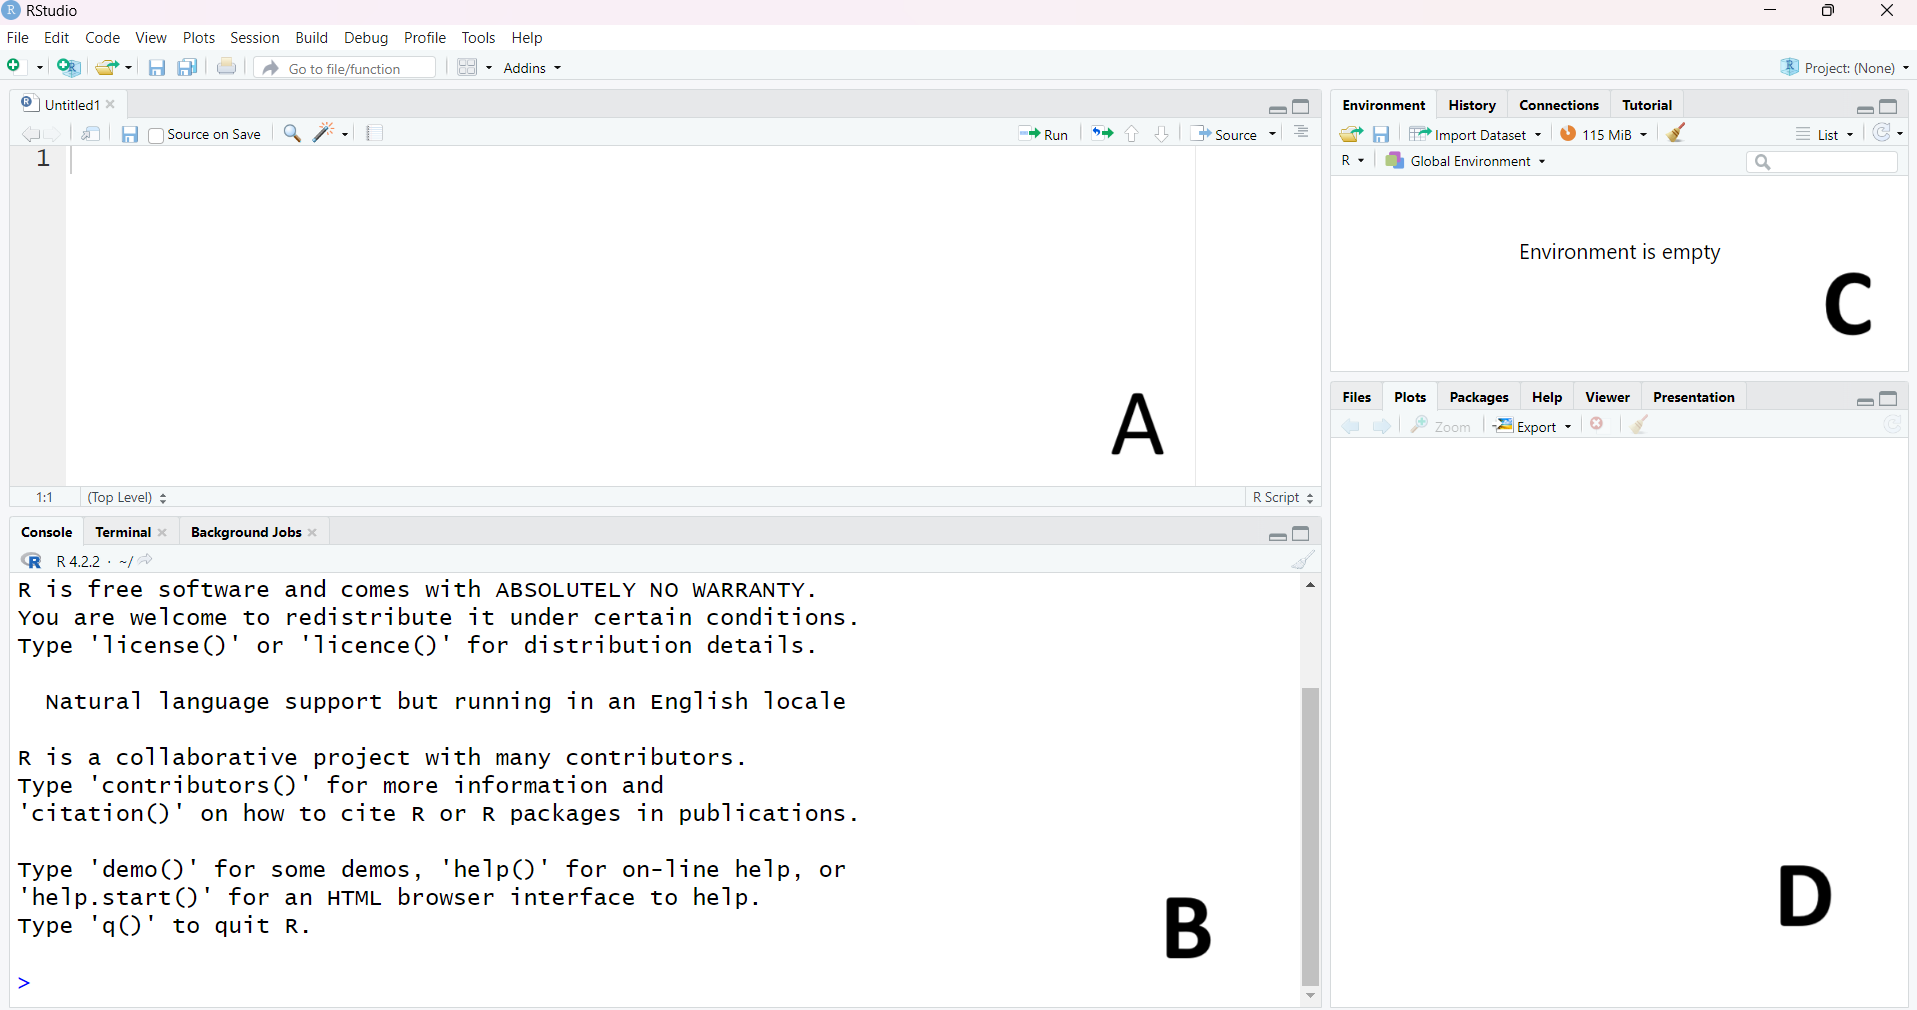
\includegraphics{img/rstudio_console.png}

}

\caption{RStudio console window}

\end{figure}%

\subsection{Window A: R script files}\label{window-a-r-script-files}

All analysis and actions in R are carried out using the R syntax
language. R script files allow us to write and edit code before running
it in the console window.

\begin{tcolorbox}[enhanced jigsaw, bottomrule=.15mm, left=2mm, leftrule=.75mm, bottomtitle=1mm, coltitle=black, colbacktitle=quarto-callout-tip-color!10!white, toptitle=1mm, arc=.35mm, breakable, title=\textcolor{quarto-callout-tip-color}{\faLightbulb}\hspace{0.5em}{Style tip}, rightrule=.15mm, toprule=.15mm, opacityback=0, opacitybacktitle=0.6, titlerule=0mm, colback=white, colframe=quarto-callout-tip-color-frame]

Limit script files to 80 characters per line to ensure it is readable.

RStudio has an option to add a margin that makes this easier to adhere
to. Under the \emph{Tools} drop-down menu, select \emph{Global options}.
Select \emph{Code} from the list on the right, then under the
\emph{Display} tab, tick the \emph{Show margin} box.

\end{tcolorbox}

If this window is not visible, create a new script file using \emph{File
-\textgreater{} New File -\textgreater{} R Script} option from the
drop-down menus or clicking the 
\includegraphics{img/new_script.png}
icon above the console and selecting `R Script'. This will open a new,
blank script file. More than one script file can be open at the same
time.

Code entered into the script file does not run automatically. To run
commands, highlight the code from the script file and click the

\includegraphics{img/run_icon.png} icon above the top right corner of
the script window (this can be carried out by pressing
\texttt{Ctrl\ +\ Enter} in Windows or \texttt{Command\ +\ Enter} on a
Mac computer). Multiple lines of code can be run at once.

The main advantage of using the script file rather than entering the
code directly into the console is that it can be saved, edited and
shared. To save a script file, use \emph{File -\textgreater{} Save
As\ldots{}} from the drop down menu, click the

\includegraphics{img/save_icon.png} icon at the top of the window, or
use the keyboard shortcut \texttt{ctrl\ +\ s} for Windows and
\texttt{command\ +\ s} for Mac. It is important to save the script files
at regular intervals to avoid losing work.

\begin{tcolorbox}[enhanced jigsaw, bottomrule=.15mm, left=2mm, leftrule=.75mm, bottomtitle=1mm, coltitle=black, colbacktitle=quarto-callout-tip-color!10!white, toptitle=1mm, arc=.35mm, breakable, title=\textcolor{quarto-callout-tip-color}{\faLightbulb}\hspace{0.5em}{Style tip}, rightrule=.15mm, toprule=.15mm, opacityback=0, opacitybacktitle=0.6, titlerule=0mm, colback=white, colframe=quarto-callout-tip-color-frame]

Script file names should be meaningful, lower case, and end in
\texttt{.R}. Avoid using special characters in file names, including
spaces. Use \texttt{\_} instead of spaces.

Where files should be run in a specific order, prefix the file name with
numbers.

\end{tcolorbox}

Past script files can be opened using \emph{File -\textgreater{} Open
File\ldots{}} from the drop-down menu, by clicking the

\includegraphics{img/open_icon.png} icon, or using the keyboard shortcut
\texttt{ctrl\ +\ o} for Windows and \texttt{command\ +\ o} for Mac, then
selecting a *.R file.

\subsection{Window B: R console}\label{window-b-r-console}

The R console window is where all commands run from the script file,
results (other than plots), and messages, such as errors, are displayed.
Commands can be written directly into the R console after the
\texttt{\textgreater{}} symbol and executed using \texttt{Enter} on the
keyboard. It is not recommended to write code directly into the console
as it is cannot be saved or replicated.

Every time a new R session is opened, details about version and
citations of R will be given by default. To clear text from the console
window, use the keyboard shortcut \texttt{control\ +\ l} (this is the
same for both Windows and Mac users). Be aware that this clears all text
from the console, including any results. Before running this command,
check that any results can be replicated within the script file.

\subsection{Window C: Environment and
history}\label{window-c-environment-and-history}

This window lists all data and objects currently loaded into R, and is
not available in the basic R software. More details on the types of
objects and how to use the Environment window are given in later
sections.

\subsection{Window D: Files, plots, packages and
help}\label{window-d-files-plots-packages-and-help}

This window has many potential uses: plots are displayed and can be
saved from here, and R help files will appear here. This window is only
available in the RStudio interface and not in the basic R package.

\section{Exercise 1}\label{exercise-1}

\begin{enumerate}
\def\labelenumi{\arabic{enumi}.}
\tightlist
\item
  Open a new script file if you have not already done so.
\item
  Save this script file into an appropriate location.
\end{enumerate}

\bookmarksetup{startatroot}

\chapter{R syntax}\label{r-syntax}

All analyses within R is carried out using syntax, the R programming
language. It is important to note that R is case-sensitive so always
ensure that you use the correct combination of upper and lower case
letters when running functions or calling objects.

Any text written in the R console or script file can be treated the same
as text from other documents or programmes: text can be highlighted,
copied and pasted to make coding more efficient.

When creating script files, it is important to ensure they are clear and
easy to read. Comments can be added to script files using the
\texttt{\#} symbol. R will ignore any text following the \texttt{\#} on
the same line.

\begin{tcolorbox}[enhanced jigsaw, bottomrule=.15mm, left=2mm, leftrule=.75mm, bottomtitle=1mm, coltitle=black, colbacktitle=quarto-callout-tip-color!10!white, toptitle=1mm, arc=.35mm, breakable, title=\textcolor{quarto-callout-tip-color}{\faLightbulb}\hspace{0.5em}{Style tip}, rightrule=.15mm, toprule=.15mm, opacityback=0, opacitybacktitle=0.6, titlerule=0mm, colback=white, colframe=quarto-callout-tip-color-frame]

Combining \texttt{\#} and \texttt{-} creates sections within a script
file, making them easier to navigate and organise.

For example:

\begin{Shaded}
\begin{Highlighting}[]
\CommentTok{\# Load data {-}{-}{-}{-}{-}{-}{-}{-}{-}{-}}

\CommentTok{\# Tidy data {-}{-}{-}{-}{-}{-}{-}{-}{-}{-}}
\end{Highlighting}
\end{Shaded}

\end{tcolorbox}

\begin{tcolorbox}[enhanced jigsaw, bottomrule=.15mm, left=2mm, leftrule=.75mm, bottomtitle=1mm, coltitle=black, colbacktitle=quarto-callout-note-color!10!white, toptitle=1mm, arc=.35mm, breakable, title=\textcolor{quarto-callout-note-color}{\faInfo}\hspace{0.5em}{Helpful hint}, rightrule=.15mm, toprule=.15mm, opacityback=0, opacitybacktitle=0.6, titlerule=0mm, colback=white, colframe=quarto-callout-note-color-frame]

To comment out chunks of code, highlight the rows and use the keyboard
shortcut \emph{ctrl + shift + c} on Windows, and \emph{Command + shift +
c} on Mac

\end{tcolorbox}

The choice of brackets in R coding is particularly important as they all
have different functions:

\begin{itemize}
\tightlist
\item
  Round brackets \texttt{(\ )} are the most commonly used as they define
  arguments of functions. Any text followed by round brackets is assumed
  to be a function and R will attempt to run it. If the name of a
  function is not followed by round brackets, R will return the
  algorithm used to create the function within the console.
\item
  Square brackets \texttt{{[}\ {]}} are used to set criteria or
  conditions within a function or object.
\item
  Curly brackets \texttt{\{\ \}} are used within loops, when creating a
  new function, and within \texttt{for} and \texttt{if} functions.
\end{itemize}

All standard notation for mathematical calculations (\texttt{+},
\texttt{-}, \texttt{*}, \texttt{/}, \texttt{\^{}}, etc.) are compatible
with R. At its simplest level, R is just a very powerful calculator!

\begin{tcolorbox}[enhanced jigsaw, bottomrule=.15mm, left=2mm, leftrule=.75mm, bottomtitle=1mm, coltitle=black, colbacktitle=quarto-callout-tip-color!10!white, toptitle=1mm, arc=.35mm, breakable, title=\textcolor{quarto-callout-tip-color}{\faLightbulb}\hspace{0.5em}{Style tip}, rightrule=.15mm, toprule=.15mm, opacityback=0, opacitybacktitle=0.6, titlerule=0mm, colback=white, colframe=quarto-callout-tip-color-frame]

Although R will work whether a space is added before/after a
mathematical operator, the
\href{https://style.tidyverse.org/syntax.html}{style guide} recommends
to add them surrounding most mathematical operations (\texttt{+},
\texttt{-}, \texttt{*}, \texttt{/}), but not around \texttt{\^{}}.

For example:

\begin{Shaded}
\begin{Highlighting}[]
\CommentTok{\# Stylish code}
\DecValTok{1959} \SpecialCharTok{{-}} \DecValTok{683}
\NormalTok{(}\DecValTok{351} \SpecialCharTok{+} \DecValTok{457}\NormalTok{)}\SpecialCharTok{\^{}}\DecValTok{2} \SpecialCharTok{{-}}\NormalTok{ (}\DecValTok{213} \SpecialCharTok{+} \DecValTok{169}\NormalTok{)}\SpecialCharTok{\^{}}\DecValTok{2}

\CommentTok{\# Un{-}stylish code}
\DecValTok{1959{-}683}
\NormalTok{(}\DecValTok{351}\SpecialCharTok{+}\DecValTok{457}\NormalTok{)}\SpecialCharTok{\^{}}\DecValTok{2} \SpecialCharTok{{-}}\NormalTok{ (}\DecValTok{213} \SpecialCharTok{+} \DecValTok{169}\NormalTok{) }\SpecialCharTok{\^{}} \DecValTok{2}
\end{Highlighting}
\end{Shaded}

\end{tcolorbox}

\section{Exercise 2}\label{exercise-2}

\begin{enumerate}
\def\labelenumi{\arabic{enumi}.}
\tightlist
\item
  Add your name and the date to the top of your script file (hint:
  comment this out so R does not try to run it)
\item
  Use R to answer to following and write the answers within the script
  file:
\end{enumerate}

\begin{enumerate}
\def\labelenumi{\alph{enumi}.}
\tightlist
\item
  \(64^2\)
\item
  \(3432 \div 8\)
\item
  \(96 \times 72\)
\end{enumerate}

\bookmarksetup{startatroot}

\chapter{R objects, functions and
packages}\label{r-objects-functions-and-packages}

\section{Objects}\label{objects}

One of the main advantages to using R over other software packages such
as SPSS is that more than one dataset can be accessed at the same time.
A collection of data stored in any format within the R session is known
as an \textbf{object}. Objects can include single numbers, single
variables, entire datasets, lists of datasets, or even tables and
graphs.

\begin{tcolorbox}[enhanced jigsaw, bottomrule=.15mm, left=2mm, leftrule=.75mm, bottomtitle=1mm, coltitle=black, colbacktitle=quarto-callout-tip-color!10!white, toptitle=1mm, arc=.35mm, breakable, title=\textcolor{quarto-callout-tip-color}{\faLightbulb}\hspace{0.5em}{Style tip}, rightrule=.15mm, toprule=.15mm, opacityback=0, opacitybacktitle=0.6, titlerule=0mm, colback=white, colframe=quarto-callout-tip-color-frame]

Object names should only contain lower case letters, numbers and
\texttt{\_} (instead of a space to separate words). The should be
meaningful and concise.

\end{tcolorbox}

Objects are defined in R using the \texttt{\textless{}-} symbol or
\texttt{=}. For example,

\begin{Shaded}
\begin{Highlighting}[]
\NormalTok{object\_1 }\OtherTok{\textless{}{-}} \DecValTok{81}
\end{Highlighting}
\end{Shaded}

Creates an object in the environment named \texttt{object\_1}, which
takes the value \texttt{81}. This will appear in the environment window
of the console (window C from the interface shown in the
\href{introduction.qmd}{introduction}).

\begin{tcolorbox}[enhanced jigsaw, bottomrule=.15mm, left=2mm, leftrule=.75mm, bottomtitle=1mm, coltitle=black, colbacktitle=quarto-callout-tip-color!10!white, toptitle=1mm, arc=.35mm, breakable, title=\textcolor{quarto-callout-tip-color}{\faLightbulb}\hspace{0.5em}{Style tip}, rightrule=.15mm, toprule=.15mm, opacityback=0, opacitybacktitle=0.6, titlerule=0mm, colback=white, colframe=quarto-callout-tip-color-frame]

Although both work, use \texttt{\textless{}-} for assignment, not
\texttt{=}.

\end{tcolorbox}

To retrieve an object, type its name into the script or console and run
it. This object can then be included in functions or operations in place
of the value assigned to it:

\begin{Shaded}
\begin{Highlighting}[]
\NormalTok{object\_1}
\end{Highlighting}
\end{Shaded}

\begin{verbatim}
[1] 81
\end{verbatim}

\begin{Shaded}
\begin{Highlighting}[]
\FunctionTok{sqrt}\NormalTok{(object\_1)}
\end{Highlighting}
\end{Shaded}

\begin{verbatim}
[1] 9
\end{verbatim}

R has some mathematical objects stored by default such as pi that can be
used in calculations.

\begin{Shaded}
\begin{Highlighting}[]
\NormalTok{pi}
\end{Highlighting}
\end{Shaded}

\begin{verbatim}
[1] 3.141593
\end{verbatim}

\section{Functions}\label{functions}

\textbf{Functions} are built-in commands that allow R users to run
analyses. All functions require the definition of arguments within round
brackets \texttt{()}. Each function requires different information and
has different arguments that can be used to customise the analysis. A
detailed list of these arguments and a description of the function can
be found in the function's associated \textbf{help file}.

\subsection{Help files}\label{help-files}

Each function that exists within R has an associated help file. RStudio
does not require an internet connection to access these help files if
the function is available in the current session of R.

To retrieve help files, enter \texttt{?} followed by the function name
into the console window, e.g \texttt{?mean}. The help file will appear
in window D of the interface shown in the
\href{intro.qmd}{introduction}.

Help files contain the following information:

\begin{itemize}
\tightlist
\item
  Description: what the function is used for
\item
  Usage: how the function is used
\item
  Arguments: required and optional arguments entered into round brackets
  necessary for the function to work
\item
  Details: relevant details about the function in question
\item
  References
\item
  See also: links to other relevant functions
\item
  Examples: example code with applications of the function
\end{itemize}

\subsection{Error and warning
messages}\label{error-and-warning-messages}

Where a function or object has not been correctly specified, or their is
some mistake in the syntax that has been sent to the console, R will
return an error message. These messages are generally informative and
include the location of the error.

The most common errors include misspelling functions or objects:

\begin{Shaded}
\begin{Highlighting}[]
\FunctionTok{sqrt}\NormalTok{(ojbect\_1)}
\end{Highlighting}
\end{Shaded}

\begin{verbatim}
Error in eval(expr, envir, enclos): object 'ojbect_1' not found
\end{verbatim}

\begin{Shaded}
\begin{Highlighting}[]
\FunctionTok{Sqrt}\NormalTok{(object\_1)}
\end{Highlighting}
\end{Shaded}

\begin{verbatim}
Error in Sqrt(object_1): could not find function "Sqrt"
\end{verbatim}

Or where an object has not yet been specified:

\begin{Shaded}
\begin{Highlighting}[]
\FunctionTok{plot}\NormalTok{(x, y)}
\end{Highlighting}
\end{Shaded}

\begin{verbatim}
Error in eval(expr, envir, enclos): object 'x' not found
\end{verbatim}

When R returns an error message, this means that the operation has been
completely halted. R may also return warning messages which look similar
to errors but does not necessarily mean the operation has been stopped.

Warnings are included to indicate that R suspects something in the
operation may be wrong and should be checked. There are occasions where
warnings can be ignored but this is only after the operation has been
checked.

\subsection{Cleaning the environment}\label{cleaning-the-environment}

To remove objects from the RStudio environment, we can use the
\texttt{rm} function. This can be combined with the \texttt{ls()}
function, which lists all objects in the environment, to remove all
objects currently loaded:

\begin{Shaded}
\begin{Highlighting}[]
\FunctionTok{rm}\NormalTok{(}\AttributeTok{list =} \FunctionTok{ls}\NormalTok{())}
\end{Highlighting}
\end{Shaded}

\begin{tcolorbox}[enhanced jigsaw, bottomrule=.15mm, left=2mm, leftrule=.75mm, bottomtitle=1mm, coltitle=black, colbacktitle=quarto-callout-warning-color!10!white, toptitle=1mm, arc=.35mm, breakable, title=\textcolor{quarto-callout-warning-color}{\faExclamationTriangle}\hspace{0.5em}{Warning}, rightrule=.15mm, toprule=.15mm, opacityback=0, opacitybacktitle=0.6, titlerule=0mm, colback=white, colframe=quarto-callout-warning-color-frame]

There are no undo and redo buttons for R syntax. The \texttt{rm}
function will permanently delete objects from the environment. The only
way to reverse this is to re-run the code that created the objects
originally from the script file.

\end{tcolorbox}

\section{Packages}\label{packages}

R packages are a collection of functions and datasets developed by R
users that expand existing R capabilities or add completely new ones.
Packages allow users to apply the most up-to-date methods shortly after
they are developed, unlike other statistical software packages that
require an entirely new version.

\subsection{Installing packages from
CRAN}\label{installing-packages-from-cran}

The quickest way to install a package in R is by using the
\texttt{install.packages} function. This sends RStudio to the online
repository of tested and verified R packages (known as
\href{https://cran.r-project.org/}{CRAN}) and downloads the package
files onto the machine you are currently working from in temporary
files. Ensure that the package you wish to install is spelled correctly
and surrounded by \texttt{\textquotesingle{}\textquotesingle{}}.

\begin{tcolorbox}[enhanced jigsaw, bottomrule=.15mm, left=2mm, leftrule=.75mm, bottomtitle=1mm, coltitle=black, colbacktitle=quarto-callout-warning-color!10!white, toptitle=1mm, arc=.35mm, breakable, title=\textcolor{quarto-callout-warning-color}{\faExclamationTriangle}\hspace{0.5em}{Warning}, rightrule=.15mm, toprule=.15mm, opacityback=0, opacitybacktitle=0.6, titlerule=0mm, colback=white, colframe=quarto-callout-warning-color-frame]

The \texttt{install.packages} function requires an internet connection,
and can take a long time if the package has a lot of dependent packages
that also need downloading.

This process should only be carried out the first time a package is used
on a machine, or when a substantial update has taken place, to download
the latest version of the package.

\end{tcolorbox}

\subsection{Loading packages to an R
session}\label{loading-packages-to-an-r-session}

Every time a new session of RStudio is opened, packages must be
reloaded. To load a package into R (and gain access to the associated
functions and data), use the \texttt{library} function.

Loading a package does not require an internet connection, but will only
work if the package has already been installed and saved onto the
computer you are working from. If you are unsure, use the function
\texttt{installed.packages} to return a list of all packages that are
loaded onto the machine you are working from.

\begin{tcolorbox}[enhanced jigsaw, bottomrule=.15mm, left=2mm, leftrule=.75mm, bottomtitle=1mm, coltitle=black, colbacktitle=quarto-callout-tip-color!10!white, toptitle=1mm, arc=.35mm, breakable, title=\textcolor{quarto-callout-tip-color}{\faLightbulb}\hspace{0.5em}{Style tip}, rightrule=.15mm, toprule=.15mm, opacityback=0, opacitybacktitle=0.6, titlerule=0mm, colback=white, colframe=quarto-callout-tip-color-frame]

Begin any script file that requires packages by loading them into the
current session. This ensures that there will be no error messages from
functions that are not available in the current session.

\end{tcolorbox}

\subsection{The pacman package}\label{the-pacman-package}

The \texttt{pacman} package is a set of package management functions
which is designed to make tasks such as installing and loading packages
simpler, and speeds up these processes. There are lots of useful
functions included in this package, but the one that we will be using in
this course is \texttt{p\_load}.

\texttt{p\_load} acts as a wrapper for the \texttt{library} function. It
first checks the computer to see whether the package(s) listed is
installed. If they are, \texttt{p\_load} loads the package(s) into the
current RStudio session. If not, it attempts to install the package(s)
from the CRAN repository.

If you have never used the \texttt{pacman} package before, run the
following code to ensure that it is installed on your machine:

\begin{Shaded}
\begin{Highlighting}[]
\FunctionTok{install.packages}\NormalTok{(}\StringTok{\textquotesingle{}pacman\textquotesingle{}}\NormalTok{)}
\end{Highlighting}
\end{Shaded}

\bookmarksetup{startatroot}

\chapter{Opening and exploring data}\label{opening-and-exploring-data}

\section{Styles of R coding}\label{styles-of-r-coding}

Up to this point, beyond the style tips sprinkled through these notes,
we have not thought about the style of R coding we will be using. There
are different approaches to R coding that we can use, they can be
thought of as different dialects of the R programming language.

The choice of R `dialect' depends on personal preference. Some prefer to
use the `base R' approach that does not rely on any packages that may
need updating, making it a more stable approach. However, base R can be
difficult to read for those not comfortable with coding.


\includegraphics{open_explore_data_files/figure-pdf/boyfriend meme-1.png}

The alternative approach that we will be adopting in this course is the
`tidyverse' approach. Tidyverse is a set of packages that have been
designed to make R coding more readable and efficient. They have been
designed with reproducibility in mind, which means there is a wealth of
online (mostly free), well-written resources available to help use these
packages. Tidyverse is also the preferred coding style of the Government
Analysis Function guidance.

If you have not done so already, install the Tidyverse packages to your
machine using the following code:

\begin{Shaded}
\begin{Highlighting}[]
\FunctionTok{install.packages}\NormalTok{(}\StringTok{\textquotesingle{}tidyverse\textquotesingle{}}\NormalTok{)}
\end{Highlighting}
\end{Shaded}

\begin{tcolorbox}[enhanced jigsaw, bottomrule=.15mm, left=2mm, leftrule=.75mm, bottomtitle=1mm, coltitle=black, colbacktitle=quarto-callout-warning-color!10!white, toptitle=1mm, arc=.35mm, breakable, title=\textcolor{quarto-callout-warning-color}{\faExclamationTriangle}\hspace{0.5em}{Warning}, rightrule=.15mm, toprule=.15mm, opacityback=0, opacitybacktitle=0.6, titlerule=0mm, colback=white, colframe=quarto-callout-warning-color-frame]

This can take a long time if you have never downloaded the tidyverse
packages before as there are many dependencies that are required.

Do not stress if you get a lot of text in the console! This is normal,
but watch out for any error messages.

\end{tcolorbox}

Once the tidyverse package is installed, we must load it into the
current working session. At the beginning of your script file add the
following syntax:

\begin{Shaded}
\begin{Highlighting}[]
\NormalTok{pacman}\SpecialCharTok{::}\FunctionTok{p\_load}\NormalTok{(tidyverse)}
\end{Highlighting}
\end{Shaded}

\begin{tcolorbox}[enhanced jigsaw, bottomrule=.15mm, left=2mm, leftrule=.75mm, bottomtitle=1mm, coltitle=black, colbacktitle=quarto-callout-tip-color!10!white, toptitle=1mm, arc=.35mm, breakable, title=\textcolor{quarto-callout-tip-color}{\faLightbulb}\hspace{0.5em}{Style tip}, rightrule=.15mm, toprule=.15mm, opacityback=0, opacitybacktitle=0.6, titlerule=0mm, colback=white, colframe=quarto-callout-tip-color-frame]

The double colon in R can be used to run a function within an installed
package without loading the entire package to an R session.

\end{tcolorbox}

\section{The working directory}\label{the-working-directory}

The working directory is a file path on your computer that R sets as the
default location when opening, saving, or exporting documents, files,
and graphics. This file path can be specified manually but setting the
working directory saves time and makes code more efficient.

The working directory can be set manually by using the \emph{Session
-\textgreater{} Set Working Directory -\textgreater{} Change
Directory\ldots{}} option from the drop-down menu, or the \texttt{setwd}
function. Both options require the directory to be specified each time R
is restarted, are sensitive to changes in folders within the file path,
and cannot be used when script files are shared between colleagues.

An alternative approach that overcomes all these issues is to create an
R project.

\subsection{R projects}\label{r-projects}

R projects are files (saved with the \texttt{.Rproj} extension) that
keep associated files (including scripts, data, and outputs) grouped
together. An R project automatically sets the working directory relative
to its current location, which makes collaborative work easier, and
avoids issues when a file path is changed.

Projects are created by using the \emph{File -\textgreater{} New
project} option from the drop-down menu, or using the

\includegraphics{img/project_icon.png} icon from the top-right corner of
the RStudio interface. Existing projects can be opened under the
\emph{File -\textgreater{} Open project\ldots{}} drop-down menu or using
the project icon.

When creating a new project, we must choose whether we are creating a
new directory or using an existing one. Usually, we will have already
set up a folder containing data or other documents related to the
analysis we plan to carry out. If this is the case, we are using an
existing directory and selecting the analysis folder as the project
directory.

\begin{tcolorbox}[enhanced jigsaw, bottomrule=.15mm, left=2mm, leftrule=.75mm, bottomtitle=1mm, coltitle=black, colbacktitle=quarto-callout-tip-color!10!white, toptitle=1mm, arc=.35mm, breakable, title=\textcolor{quarto-callout-tip-color}{\faLightbulb}\hspace{0.5em}{Style tip}, rightrule=.15mm, toprule=.15mm, opacityback=0, opacitybacktitle=0.6, titlerule=0mm, colback=white, colframe=quarto-callout-tip-color-frame]

Have a clear order to your analysis folder. Consider creating separate
folders within a project for input and output data, documentation, and
outputs such as graphs or tables.

\end{tcolorbox}

\section{Loading data}\label{loading-data}

To ensure our code is collaborative and reproducible, we should strive
to store data in formats that can be used across multiple platforms. One
of the best ways to do this is to store data as a comma-delimited file
(.csv). CSV files can be opened by a range of different softwares
(including R, SPSS, STATA and excel), and base R can be used to open
these files without requiring additional packages.

Unfortunately, we are not always able to choose the format that data are
stored in. For example, the English Housing Survey (EHS) data is stored
as a .sav (SPSS) data file. Fortunately for us, R has a wide range of
packages that have been developed to load data from every conceivable
format.

The package that we will be using the load SPSS data is the
\texttt{haven} package. To ensure this is loaded in at the beginning of
each session, adapt the previous \texttt{p\_load} function:

\begin{Shaded}
\begin{Highlighting}[]
\NormalTok{pacman}\SpecialCharTok{::}\FunctionTok{p\_load}\NormalTok{(tidyverse, haven)}
\end{Highlighting}
\end{Shaded}

To avoid any errors arising from spelling mistakes, we can use the
\texttt{list.files} function, which returns a list of files and folders
from the current working directory. The file names can be copied from
the console and pasted into the script file. As the data are saved in a
folder within the working directory, we add the argument
\texttt{path\ =} to specify the folder we want to list files from.

\begin{Shaded}
\begin{Highlighting}[]
\FunctionTok{list.files}\NormalTok{(}\AttributeTok{path =} \StringTok{"data"}\NormalTok{)}
\end{Highlighting}
\end{Shaded}

\begin{verbatim}
[1] "Detailed_forecast_tables_Economy_March_2024.xlsx"
[2] "generalfs21_EUL.sav"                             
[3] "interviewfs21_EUL.sav"                           
\end{verbatim}

The first data set we will load is the\texttt{generalfs21\_EUL.sav}
file. This contains general information taken from the English Housing
Survey (EHS) from 2021, including a unique identifier, the responders'
region, and the tenure type.

The EHS data can be loaded into R using the \texttt{read\_spss}
function, and saved as an object using the \texttt{\textless{}-} symbol:

\begin{Shaded}
\begin{Highlighting}[]
\NormalTok{ehs\_general }\OtherTok{\textless{}{-}} \FunctionTok{read\_spss}\NormalTok{(}\AttributeTok{file =} \StringTok{"Data/generalfs21\_EUL.sav"}\NormalTok{)}
\end{Highlighting}
\end{Shaded}

The imported data will appear in the environment with its given name.
The contents of the object can be viewed by clicking on the object name
in the environment, opening a tab next to script files. This window is a
preview so cannot be edited here.

Some useful functions that can be used to explore a dataset include:

\begin{Shaded}
\begin{Highlighting}[]
\CommentTok{\# Return variable names}
\FunctionTok{names}\NormalTok{(ehs\_general)}
\end{Highlighting}
\end{Shaded}

\begin{verbatim}
[1] "serialanon" "aagfh21"    "paired"     "tenure8x"   "tenure4x"  
[6] "tenure2x"   "gorehs"     "region3x"   "govreg1"   
\end{verbatim}

\begin{Shaded}
\begin{Highlighting}[]
\CommentTok{\# Returns the first 6 rows}
\FunctionTok{head}\NormalTok{(ehs\_general)}
\end{Highlighting}
\end{Shaded}

\begin{verbatim}
# A tibble: 6 x 9
  serialanon  aagfh21   paired      tenure8x tenure4x tenure2x gorehs   region3x
  <dbl+lbl>   <dbl+lbl> <dbl+lbl>   <dbl+lb> <dbl+lb> <dbl+lb> <dbl+lb> <dbl+lb>
1 20220000001 3934.     1 [Paired]  1 [owne~ 1 [owne~ 1 [Priv~  7 [Eas~ 3 [Rest~
2 20220000005 1580.     1 [Paired]  1 [owne~ 1 [owne~ 1 [Priv~ 10 [Sou~ 3 [Rest~
3 20220000006 3360.     1 [Paired]  1 [owne~ 1 [owne~ 1 [Priv~  6 [Wes~ 3 [Rest~
4 20220000012 1368.     0 [Not pai~ 1 [owne~ 1 [owne~ 1 [Priv~  5 [Eas~ 3 [Rest~
5 20220000013 9847.     1 [Paired]  1 [owne~ 1 [owne~ 1 [Priv~ 10 [Sou~ 3 [Rest~
6 20220000017 3262.     0 [Not pai~ 1 [owne~ 1 [owne~ 1 [Priv~  6 [Wes~ 3 [Rest~
# i 1 more variable: govreg1 <dbl+lbl>
\end{verbatim}

\begin{Shaded}
\begin{Highlighting}[]
\CommentTok{\# Returns the last 6 rows}
\FunctionTok{tail}\NormalTok{(ehs\_general)}
\end{Highlighting}
\end{Shaded}

\begin{verbatim}
# A tibble: 6 x 9
  serialanon  aagfh21   paired      tenure8x tenure4x tenure2x gorehs   region3x
  <dbl+lbl>   <dbl+lbl> <dbl+lbl>   <dbl+lb> <dbl+lb> <dbl+lb> <dbl+lb> <dbl+lb>
1 20220031393  262.     0 [Not pai~ 3 [loca~ 3 [loca~ 2 [Soci~  7 [Eas~ 3 [Rest~
2 20220031396 5741.     1 [Paired]  1 [owne~ 1 [owne~ 1 [Priv~  6 [Wes~ 3 [Rest~
3 20220031401 1579.     0 [Not pai~ 1 [owne~ 1 [owne~ 1 [Priv~  6 [Wes~ 3 [Rest~
4 20220031402 2178.     0 [Not pai~ 1 [owne~ 1 [owne~ 1 [Priv~  9 [Sou~ 2 [Lond~
5 20220031408 1133.     1 [Paired]  1 [owne~ 1 [owne~ 1 [Priv~ 10 [Sou~ 3 [Rest~
6 20220031409 1879.     1 [Paired]  1 [owne~ 1 [owne~ 1 [Priv~ 10 [Sou~ 3 [Rest~
# i 1 more variable: govreg1 <dbl+lbl>
\end{verbatim}

\begin{Shaded}
\begin{Highlighting}[]
\CommentTok{\# Gives information about the structure of an object (including variable types)}
\FunctionTok{str}\NormalTok{(ehs\_general)}
\end{Highlighting}
\end{Shaded}

\begin{verbatim}
tibble [9,752 x 9] (S3: tbl_df/tbl/data.frame)
 $ serialanon: dbl+lbl [1:9752] 2.02e+10, 2.02e+10, 2.02e+10, 2.02e+10, 2.02e+10, 2.0...
   ..@ label        : chr "Key variable: unique archived identifier"
   ..@ format.spss  : chr "F11.0"
   ..@ display_width: int 13
   ..@ labels       : Named num [1:2] -9 -8
   .. ..- attr(*, "names")= chr [1:2] "Does not apply" "No Answer"
 $ aagfh21   : dbl+lbl [1:9752] 3934, 1580, 3360, 1368, 9847, 3262, 6584,  389, 4193,...
   ..@ label        : chr "Household weight 2021"
   ..@ format.spss  : chr "F8.2"
   ..@ display_width: int 10
   ..@ labels       : Named num [1:2] -9 -8
   .. ..- attr(*, "names")= chr [1:2] "Does not apply" "No answer"
 $ paired    : dbl+lbl [1:9752] 1, 1, 1, 0, 1, 0, 0, 0, 1, 1, 0, 1, 1, 1, 1, 0, 0, 1,...
   ..@ label      : chr "Whether paired sample case"
   ..@ format.spss: chr "F3.0"
   ..@ labels     : Named num [1:4] -9 -8 0 1
   .. ..- attr(*, "names")= chr [1:4] "Does not apply" "No Answer" "Not paired" "Paired"
 $ tenure8x  : dbl+lbl [1:9752] 1, 1, 1, 1, 1, 1, 1, 1, 2, 1, 1, 4, 1, 4, 1, 1, 2, 4,...
   ..@ label        : chr "Tenure with vacancy"
   ..@ format.spss  : chr "F2.0"
   ..@ display_width: int 10
   ..@ labels       : Named num [1:10] -9 -8 1 2 3 4 5 6 7 8
   .. ..- attr(*, "names")= chr [1:10] "Does not apply" "No Answer" "owner occupied - occupied" "private rented - occupied" ...
 $ tenure4x  : dbl+lbl [1:9752] 1, 1, 1, 1, 1, 1, 1, 1, 2, 1, 1, 4, 1, 4, 1, 1, 2, 4,...
   ..@ label        : chr "Tenure"
   ..@ format.spss  : chr "F2.0"
   ..@ display_width: int 10
   ..@ labels       : Named num [1:6] -9 -8 1 2 3 4
   .. ..- attr(*, "names")= chr [1:6] "Does not apply" "No Answer" "owner occupied" "private rented" ...
 $ tenure2x  : dbl+lbl [1:9752] 1, 1, 1, 1, 1, 1, 1, 1, 1, 1, 1, 2, 1, 2, 1, 1, 1, 2,...
   ..@ label        : chr "Tenure"
   ..@ format.spss  : chr "F2.0"
   ..@ display_width: int 10
   ..@ labels       : Named num [1:4] -9 -8 1 2
   .. ..- attr(*, "names")= chr [1:4] "Does not apply" "No Answer" "Private" "Social"
 $ gorehs    : dbl+lbl [1:9752]  7, 10,  6,  5, 10,  6,  4, 10,  7,  2, 10,  2,  2,  ...
   ..@ label      : chr "Government Office Region EHS version"
   ..@ format.spss: chr "F2.0"
   ..@ labels     : Named num [1:11] -9 -8 1 2 4 5 6 7 8 9 ...
   .. ..- attr(*, "names")= chr [1:11] "Does not apply" "No answer" "North East" "North West" ...
 $ region3x  : dbl+lbl [1:9752] 3, 3, 3, 3, 3, 3, 1, 3, 3, 1, 3, 1, 1, 3, 1, 2, 3, 1,...
   ..@ label        : chr "Overall region of England"
   ..@ format.spss  : chr "F2.0"
   ..@ display_width: int 10
   ..@ labels       : Named num [1:5] -9 -8 1 2 3
   .. ..- attr(*, "names")= chr [1:5] "Does not apply" "No Answer" "Northern regions" "London and South East regions" ...
 $ govreg1   : dbl+lbl [1:9752] 4, 4, 2, 2, 4, 2, 1, 4, 4, 1, 4, 1, 1, 2, 1, 4, 4, 1,...
   ..@ label        : chr "Government office Region, grouped"
   ..@ format.spss  : chr "F2.0"
   ..@ display_width: int 9
   ..@ labels       : Named num [1:6] -9 -8 1 2 3 4
   .. ..- attr(*, "names")= chr [1:6] "Does not apply" "No Answer" "North" "Midlands" ...
 - attr(*, "notes")= chr [1:6] "This third delivery file (interviewfs21.sav)" "was updated on 29/11/22" "   (Entered 01-Dec-2022)" "This third delivery file (interviewfs21.sav)" ...
\end{verbatim}

The \texttt{str} function tells us that this object is a
\texttt{tibble}. This is tidyverse language for a data set (in base R,
it is known as a \texttt{data.frame}). All variables are recognised as
\texttt{dbl\ +\ lbl}, or labelled double variables. Double is tidyverse
language for numeric data, and labels are taken from the original SPSS
data.

It is important to check that R has correctly recognised variable type
when data are loaded, before generating any visualisations or analysis.
If variables are incorrectly specified, this could either lead to errors
or invalid analyses. We will see how to change variables types later in
this chapter.

The variables in this tibble contain additional information, stored as
\texttt{attributes}. Data imported from other sources do not typically
include these attributes by default, but these are able to uphold any
information that was stored in the `Variable view' window of SPSS.

\section{Selecting variables}\label{selecting-variables}

Often, we will not need every variable in a downloaded dataset to carry
out an analysis, and we may wish to create a smaller analysis tibble. We
may also wish to select individual variables from the tibble to apply
functions to them without including the entire dataset.

To select one or more variable and return them as a new tibble, we can
use the \texttt{select} function from tidyverse's \texttt{dplyr}
package.

For example, we do not need all the variables contained in the EHS
general dataset. The variables we are interested in keeping are the
unique identifier variables (\texttt{serialanon}), the survey weights
(\texttt{aagfh21}), the tenure type response with 4 options
(\texttt{tenure4x}), and the Government office region
(\texttt{govreg1}):

\begin{Shaded}
\begin{Highlighting}[]
\CommentTok{\# Variables can be selected using their names}
\FunctionTok{select}\NormalTok{(ehs\_general, serialanon, aagfh21, tenure4x, gorehs)}
\end{Highlighting}
\end{Shaded}

\begin{verbatim}
# A tibble: 9,752 x 4
   serialanon  aagfh21   tenure4x           gorehs                       
   <dbl+lbl>   <dbl+lbl> <dbl+lbl>          <dbl+lbl>                    
 1 20220000001 3934.     1 [owner occupied]  7 [East]                    
 2 20220000005 1580.     1 [owner occupied] 10 [South West]              
 3 20220000006 3360.     1 [owner occupied]  6 [West Midlands]           
 4 20220000012 1368.     1 [owner occupied]  5 [East Midlands]           
 5 20220000013 9847.     1 [owner occupied] 10 [South West]              
 6 20220000017 3262.     1 [owner occupied]  6 [West Midlands]           
 7 20220000022 6584.     1 [owner occupied]  4 [Yorkshire and the Humber]
 8 20220000025  389.     1 [owner occupied] 10 [South West]              
 9 20220000026 4193.     2 [private rented]  7 [East]                    
10 20220000027 3589.     1 [owner occupied]  2 [North West]              
# i 9,742 more rows
\end{verbatim}

\begin{Shaded}
\begin{Highlighting}[]
\CommentTok{\# Or their column number}
\FunctionTok{select}\NormalTok{(ehs\_general, }\DecValTok{1}\NormalTok{, }\DecValTok{2}\NormalTok{, }\DecValTok{5}\NormalTok{, }\DecValTok{7}\NormalTok{)}
\end{Highlighting}
\end{Shaded}

\begin{verbatim}
# A tibble: 9,752 x 4
   serialanon  aagfh21   tenure4x           gorehs                       
   <dbl+lbl>   <dbl+lbl> <dbl+lbl>          <dbl+lbl>                    
 1 20220000001 3934.     1 [owner occupied]  7 [East]                    
 2 20220000005 1580.     1 [owner occupied] 10 [South West]              
 3 20220000006 3360.     1 [owner occupied]  6 [West Midlands]           
 4 20220000012 1368.     1 [owner occupied]  5 [East Midlands]           
 5 20220000013 9847.     1 [owner occupied] 10 [South West]              
 6 20220000017 3262.     1 [owner occupied]  6 [West Midlands]           
 7 20220000022 6584.     1 [owner occupied]  4 [Yorkshire and the Humber]
 8 20220000025  389.     1 [owner occupied] 10 [South West]              
 9 20220000026 4193.     2 [private rented]  7 [East]                    
10 20220000027 3589.     1 [owner occupied]  2 [North West]              
# i 9,742 more rows
\end{verbatim}

The \texttt{select} function can also be combined with a number of
`selection helper' functions that help us select variables based on
naming conventions:

\begin{itemize}
\tightlist
\item
  \texttt{starts\_with("xyz")} returns all variables with names
  beginning \texttt{xyz}
\item
  \texttt{ends\_with("xyz")} returns all variables with names ending
  \texttt{xyz}
\item
  \texttt{contains("xyz")} returns all variables that have \texttt{xyz}
  within their name
\end{itemize}

Or based on whether they match a condition:

\begin{itemize}
\tightlist
\item
  \texttt{where(is.numeric)} returns all variables that are classed as
  numeric
\end{itemize}

For a full list of these selection helpers, access the helpfile using
\texttt{?tidyr\_tidy\_select}.

The \texttt{select} function can also be used to remove variables from a
tibble by adding a \texttt{-} before the variable name or number. For
example, to return the EHS general dataset without the unique identifier
variable, we use:

\begin{Shaded}
\begin{Highlighting}[]
\FunctionTok{select}\NormalTok{(ehs\_general, }\SpecialCharTok{{-}}\NormalTok{serialanon)}
\end{Highlighting}
\end{Shaded}

\begin{verbatim}
# A tibble: 9,752 x 8
   aagfh21   paired         tenure8x tenure4x tenure2x gorehs   region3x govreg1
   <dbl+lbl> <dbl+lbl>      <dbl+lb> <dbl+lb> <dbl+lb> <dbl+lb> <dbl+lb> <dbl+l>
 1 3934.     1 [Paired]     1 [owne~ 1 [owne~ 1 [Priv~  7 [Eas~ 3 [Rest~ 4 [Res~
 2 1580.     1 [Paired]     1 [owne~ 1 [owne~ 1 [Priv~ 10 [Sou~ 3 [Rest~ 4 [Res~
 3 3360.     1 [Paired]     1 [owne~ 1 [owne~ 1 [Priv~  6 [Wes~ 3 [Rest~ 2 [Mid~
 4 1368.     0 [Not paired] 1 [owne~ 1 [owne~ 1 [Priv~  5 [Eas~ 3 [Rest~ 2 [Mid~
 5 9847.     1 [Paired]     1 [owne~ 1 [owne~ 1 [Priv~ 10 [Sou~ 3 [Rest~ 4 [Res~
 6 3262.     0 [Not paired] 1 [owne~ 1 [owne~ 1 [Priv~  6 [Wes~ 3 [Rest~ 2 [Mid~
 7 6584.     0 [Not paired] 1 [owne~ 1 [owne~ 1 [Priv~  4 [Yor~ 1 [Nort~ 1 [Nor~
 8  389.     0 [Not paired] 1 [owne~ 1 [owne~ 1 [Priv~ 10 [Sou~ 3 [Rest~ 4 [Res~
 9 4193.     1 [Paired]     2 [priv~ 2 [priv~ 1 [Priv~  7 [Eas~ 3 [Rest~ 4 [Res~
10 3589.     1 [Paired]     1 [owne~ 1 [owne~ 1 [Priv~  2 [Nor~ 1 [Nort~ 1 [Nor~
# i 9,742 more rows
\end{verbatim}

After making changes to the analysis dataset, it is useful to save this
data separately to the original raw data. This can be done using the
\texttt{write\_csv} function.

\begin{Shaded}
\begin{Highlighting}[]
\NormalTok{ehs\_general\_reduced }\OtherTok{\textless{}{-}} \FunctionTok{select}\NormalTok{(ehs\_general, serialanon, aagfh21, tenure4x, gorehs)}
\end{Highlighting}
\end{Shaded}

\begin{Shaded}
\begin{Highlighting}[]
\FunctionTok{write\_csv}\NormalTok{(ehs\_general\_reduced, }\AttributeTok{file =} \StringTok{"ehs\_general\_reduced.csv"}\NormalTok{)}
\end{Highlighting}
\end{Shaded}

\begin{tcolorbox}[enhanced jigsaw, bottomrule=.15mm, left=2mm, leftrule=.75mm, bottomtitle=1mm, coltitle=black, colbacktitle=quarto-callout-warning-color!10!white, toptitle=1mm, arc=.35mm, breakable, title=\textcolor{quarto-callout-warning-color}{\faExclamationTriangle}\hspace{0.5em}{Warning}, rightrule=.15mm, toprule=.15mm, opacityback=0, opacitybacktitle=0.6, titlerule=0mm, colback=white, colframe=quarto-callout-warning-color-frame]

When saving updated tibbles as files, use a different file name to the
original raw data. Using the same name will overwrite the original file.
We always want a copy of the original in case of any errors or issues.

\end{tcolorbox}

The \texttt{select} function returns variables as a tibble object.
However, some functions, for example summary functions from base R,
require data in the form of a \texttt{vector}. Vectors are lists of
numbers with no formal structure, unlike a tibble which is structured to
have rows and columns. To return a single variable as a vector, we can
use the \texttt{\$} symbol between the data name and the variable to
return:

\begin{Shaded}
\begin{Highlighting}[]
\NormalTok{ehs\_general\_reduced}\SpecialCharTok{$}\NormalTok{aagfh21}
\end{Highlighting}
\end{Shaded}

\section{Filtering data}\label{filtering-data}

The \texttt{filter} function, from tidyverse's \texttt{dplyr} package
allows us to return subgroups of the data based on conditional
statements. These conditional statements can include mathematical
operators, e.g.~\texttt{\textless{}=} (less than or equal to),
\texttt{==} (is equal to), and \texttt{!=} (is not equal to), or can be
based on conditional functions, e.g.~\texttt{is.na(variable)} (is
missing), \texttt{between(a,\ b)} (number lies between a and b). A list
of these conditional statements can be found in the help file using
\texttt{?filter}.

For example, we may wish to return rows from the EHS dataset that were
privately rented. To check which number refers to privately rented, we
can check the \texttt{labels} attribute of the \texttt{tenure4x}
variable which shows the labels from the SPSS file:

\begin{Shaded}
\begin{Highlighting}[]
\FunctionTok{attributes}\NormalTok{(ehs\_general\_reduced}\SpecialCharTok{$}\NormalTok{tenure4x)}\SpecialCharTok{$}\NormalTok{labels}
\end{Highlighting}
\end{Shaded}

\begin{verbatim}
     Does not apply           No Answer      owner occupied      private rented 
                 -9                  -8                   1                   2 
    local authority housing association 
                  3                   4 
\end{verbatim}

Private rented is given by a 2 in the current dataset, therefore our
conditional statement will return rows where the \texttt{tenure4x}
variable takes the value 2.

\begin{Shaded}
\begin{Highlighting}[]
\FunctionTok{filter}\NormalTok{(ehs\_general\_reduced, tenure4x }\SpecialCharTok{==} \DecValTok{2}\NormalTok{)}
\end{Highlighting}
\end{Shaded}

\begin{verbatim}
# A tibble: 1,735 x 4
   serialanon  aagfh21   tenure4x           gorehs                       
   <dbl+lbl>   <dbl+lbl> <dbl+lbl>          <dbl+lbl>                    
 1 20220000026 4193.     2 [private rented]  7 [East]                    
 2 20220000039  423.     2 [private rented]  7 [East]                    
 3 20220000075 1017.     2 [private rented]  7 [East]                    
 4 20220000092 1554.     2 [private rented]  7 [East]                    
 5 20220000113 5254.     2 [private rented]  8 [London]                  
 6 20220000132 7609.     2 [private rented]  4 [Yorkshire and the Humber]
 7 20220000134  775.     2 [private rented]  5 [East Midlands]           
 8 20220000135 1313.     2 [private rented]  1 [North East]              
 9 20220000187 1528.     2 [private rented]  8 [London]                  
10 20220000198  557.     2 [private rented] 10 [South West]              
# i 1,725 more rows
\end{verbatim}

Multiple conditional statements can be added to the same function by
separating them with a comma \texttt{,}. To return all respondents that
lived in privately rented accommodation in the North East, we can extend
the previous filter statement:

\begin{Shaded}
\begin{Highlighting}[]
\FunctionTok{attributes}\NormalTok{(ehs\_general\_reduced}\SpecialCharTok{$}\NormalTok{gorehs)}\SpecialCharTok{$}\NormalTok{labels}
\end{Highlighting}
\end{Shaded}

\begin{verbatim}
          Does not apply                No answer               North East 
                      -9                       -8                        1 
              North West Yorkshire and the Humber            East Midlands 
                       2                        4                        5 
           West Midlands                     East                   London 
                       6                        7                        8 
              South East               South West 
                       9                       10 
\end{verbatim}

\begin{Shaded}
\begin{Highlighting}[]
\CommentTok{\# North East is region 1}
\FunctionTok{filter}\NormalTok{(ehs\_general\_reduced, tenure4x }\SpecialCharTok{==} \DecValTok{2}\NormalTok{, gorehs }\SpecialCharTok{==} \DecValTok{1}\NormalTok{)}
\end{Highlighting}
\end{Shaded}

\begin{verbatim}
# A tibble: 76 x 4
   serialanon  aagfh21   tenure4x           gorehs        
   <dbl+lbl>   <dbl+lbl> <dbl+lbl>          <dbl+lbl>     
 1 20220000135  1313.    2 [private rented] 1 [North East]
 2 20220001633  3849.    2 [private rented] 1 [North East]
 3 20220002101  1016.    2 [private rented] 1 [North East]
 4 20220002817   323.    2 [private rented] 1 [North East]
 5 20220003959  2800.    2 [private rented] 1 [North East]
 6 20220004183   636.    2 [private rented] 1 [North East]
 7 20220005151 10707.    2 [private rented] 1 [North East]
 8 20220005393  2189.    2 [private rented] 1 [North East]
 9 20220005697  2059.    2 [private rented] 1 [North East]
10 20220005754   625.    2 [private rented] 1 [North East]
# i 66 more rows
\end{verbatim}

\section{Pipes}\label{pipes}

When creating an analysis-ready dataset, we often want to combine
functions such as \texttt{select} and \texttt{filter}. Previously, these
would need to be carried out separately and a new object would need to
be created or overwritten at each step, clogging up the environment.

In tidyverse, we combine functions within a single process using the
`pipe' symbol \texttt{\%\textgreater{}\%}, which is read as `and then'
within the code. For example, if we wanted to just select the unique
identifiers of respondents that were privately renting in the North
East, we could do this in a single process:

\begin{Shaded}
\begin{Highlighting}[]
\NormalTok{ehs\_general\_reduced }\SpecialCharTok{\%\textgreater{}\%} 
  \FunctionTok{filter}\NormalTok{(tenure4x }\SpecialCharTok{==} \DecValTok{2}\NormalTok{, gorehs }\SpecialCharTok{==} \DecValTok{1}\NormalTok{) }\SpecialCharTok{\%\textgreater{}\%} 
  \FunctionTok{select}\NormalTok{(serialanon)}
\end{Highlighting}
\end{Shaded}

\begin{verbatim}
# A tibble: 76 x 1
   serialanon 
   <dbl+lbl>  
 1 20220000135
 2 20220001633
 3 20220002101
 4 20220002817
 5 20220003959
 6 20220004183
 7 20220005151
 8 20220005393
 9 20220005697
10 20220005754
# i 66 more rows
\end{verbatim}

\begin{tcolorbox}[enhanced jigsaw, bottomrule=.15mm, left=2mm, leftrule=.75mm, bottomtitle=1mm, coltitle=black, colbacktitle=quarto-callout-tip-color!10!white, toptitle=1mm, arc=.35mm, breakable, title=\textcolor{quarto-callout-tip-color}{\faLightbulb}\hspace{0.5em}{Style tips}, rightrule=.15mm, toprule=.15mm, opacityback=0, opacitybacktitle=0.6, titlerule=0mm, colback=white, colframe=quarto-callout-tip-color-frame]

When combining multiple functions within a process using pipes, it is
good practice to start the code with the data and pipe that into the
functions, rather than including it in the function itself.

\end{tcolorbox}

\begin{tcolorbox}[enhanced jigsaw, bottomrule=.15mm, left=2mm, leftrule=.75mm, bottomtitle=1mm, coltitle=black, colbacktitle=quarto-callout-note-color!10!white, toptitle=1mm, arc=.35mm, breakable, title=\textcolor{quarto-callout-note-color}{\faInfo}\hspace{0.5em}{Helpful hint}, rightrule=.15mm, toprule=.15mm, opacityback=0, opacitybacktitle=0.6, titlerule=0mm, colback=white, colframe=quarto-callout-note-color-frame]

Rather than typing out pipes every time, use the keyboard shortcut
\emph{ctrl + shift + m} for Windows and \emph{Command + shift + m} for
Mac.

\end{tcolorbox}

\section{Creating new variables}\label{creating-new-variables}

The function \texttt{mutate} from tidyverse's \texttt{dplyr} package
allows us to add new variables to a dataset. We can add multiple
variables within the same function, separating each with a comma
\texttt{,}.

The \texttt{mutate} function is helpful when variable types are not
correctly specified by R when they are read in. For example, the region
and tenancy type variables in the \texttt{ehs\_general\_reduced} tibble
are categorical variables but are currently recognised as numeric.

Categorical variables in R are known as \textbf{factors}. These factors
can be ordered and can have labels assigned to different levels. To
convert an existing variable to a factor, we can use the \texttt{factor}
or \texttt{as\_factor} functions. Here, we can combine the
\texttt{mutate} and \texttt{as\_factor} functions to convert tenancy
type and region to factors:

\begin{Shaded}
\begin{Highlighting}[]
\NormalTok{ehs\_general\_reduced }\OtherTok{\textless{}{-}} \FunctionTok{mutate}\NormalTok{(ehs\_general\_reduced,}
                              \AttributeTok{tenancy\_type =} \FunctionTok{as\_factor}\NormalTok{(tenure4x),}
                              \AttributeTok{region =} \FunctionTok{as\_factor}\NormalTok{(gorehs))}
\end{Highlighting}
\end{Shaded}

\begin{tcolorbox}[enhanced jigsaw, bottomrule=.15mm, left=2mm, leftrule=.75mm, bottomtitle=1mm, coltitle=black, colbacktitle=quarto-callout-note-color!10!white, toptitle=1mm, arc=.35mm, breakable, title=\textcolor{quarto-callout-note-color}{\faInfo}\hspace{0.5em}{Note}, rightrule=.15mm, toprule=.15mm, opacityback=0, opacitybacktitle=0.6, titlerule=0mm, colback=white, colframe=quarto-callout-note-color-frame]

As this data was taken from an SPSS file that had labels attached to the
grouped variables, we do not need to specify these within the
\texttt{as\_factor} function.

When the variables do not have this labelling structure already, they
will need to be added using the \texttt{label} argument of the
\texttt{factor} function (see \texttt{?factor} for more information).

\end{tcolorbox}

The \texttt{mutate} function can also be used to convert numeric
variables into an ordered categorical variable, and can be used to
transform variables using mathematical functions. For example, we can
create two new variables, first giving the square root of the weighting
variable, and second grouping the weighting variable into three
categories (low: \(< 1000\), medium: \(1000 \leq\) \texttt{aagfh21}
\(< 5000\), high: \(\geq 5000\)):

\begin{Shaded}
\begin{Highlighting}[]
\NormalTok{ehs\_general\_reduced }\OtherTok{\textless{}{-}} \FunctionTok{mutate}\NormalTok{(ehs\_general\_reduced,}
                              \AttributeTok{weighting\_sqrt =} \FunctionTok{sqrt}\NormalTok{(aagfh21),}
                              \AttributeTok{weighting\_fct =} \FunctionTok{cut}\NormalTok{(aagfh21, }
                                                  \AttributeTok{breaks =} \FunctionTok{c}\NormalTok{(}\DecValTok{0}\NormalTok{, }\DecValTok{1000}\NormalTok{, }\DecValTok{5000}\NormalTok{, }\ConstantTok{Inf}\NormalTok{),}
                                                  \AttributeTok{right =} \ConstantTok{TRUE}\NormalTok{,}
                                                  \AttributeTok{labels =} \FunctionTok{c}\NormalTok{(}\StringTok{"Low"}\NormalTok{, }\StringTok{"Medium"}\NormalTok{,}
                                                              \StringTok{"High"}\NormalTok{)))}
\end{Highlighting}
\end{Shaded}

\begin{tcolorbox}[enhanced jigsaw, bottomrule=.15mm, left=2mm, leftrule=.75mm, bottomtitle=1mm, coltitle=black, colbacktitle=quarto-callout-note-color!10!white, toptitle=1mm, arc=.35mm, breakable, title=\textcolor{quarto-callout-note-color}{\faInfo}\hspace{0.5em}{Helpful hint}, rightrule=.15mm, toprule=.15mm, opacityback=0, opacitybacktitle=0.6, titlerule=0mm, colback=white, colframe=quarto-callout-note-color-frame]

The \texttt{c} function takes a list of values separated by commas and
returns them as a \texttt{vector}. This is useful when a function
argument requires multiple values (and we don't want R to move onto the
next argument, which is what a comma inside functions usually means).

\end{tcolorbox}

\section{\texorpdfstring{Other useful \texttt{dplyr}
functions}{Other useful dplyr functions}}\label{other-useful-dplyr-functions}

To ensure our code follows the
\href{https://style.tidyverse.org/}{tidyverse style guide}, variable
names should be concise, \emph{informative}, and contain no special
charaters (other than \texttt{\_}). The original variable names given in
the original EHS data were definitely not stylish! To change names in a
dataset, we can use the \texttt{rename} function:

\begin{Shaded}
\begin{Highlighting}[]
\NormalTok{ehs\_general\_reduced }\OtherTok{\textless{}{-}} \FunctionTok{rename}\NormalTok{(ehs\_general\_reduced,}
                              \AttributeTok{id =}\NormalTok{ serialanon,}
                              \AttributeTok{weighting =}\NormalTok{ aagfh21)}
\end{Highlighting}
\end{Shaded}

For more useful data exploration and manipulation functions from the
\texttt{dplyr} package, I would recommending taking a look at the
\textbf{vignette} associated with the package (a long-form version of a
help file):

\texttt{vignette("dplyr")}

Or look at the \texttt{dplyr}
\href{https://rstudio.github.io/cheatsheets/data-transformation.pdf}{cheatsheet}.

\section{A smooth process to the analysis
dataset}\label{a-smooth-process-to-the-analysis-dataset}

Our EHS analysis dataset has been created haphazardly through this
chapter to demostrate each step separately. In reality, we would load
this data and manipulate it in one process, separating steps by pipes
\texttt{\%\textgreater{}\%}.

The code below takes the data from its saw form (the .sav file) and
transforms it into a clean dataset that we will be using for the rest of
the course:

\begin{Shaded}
\begin{Highlighting}[]
\CommentTok{\# Step 1: load the dataset into R and attach as an object}
\NormalTok{ehs\_general\_tidy }\OtherTok{\textless{}{-}} \FunctionTok{read\_spss}\NormalTok{(}\AttributeTok{file =} \StringTok{"Data/generalfs21\_EUL.sav"}\NormalTok{) }\SpecialCharTok{\%\textgreater{}\%} 
\CommentTok{\# Step 2: convert grouping variables into factors}
                    \FunctionTok{mutate}\NormalTok{(}\AttributeTok{tenure\_type =} \FunctionTok{as\_factor}\NormalTok{(tenure4x),}
                           \AttributeTok{region =} \FunctionTok{as\_factor}\NormalTok{(gorehs)) }\SpecialCharTok{\%\textgreater{}\%} 
\CommentTok{\# Step 3: rename other variables to avoid confusion}
                    \FunctionTok{rename}\NormalTok{(}\AttributeTok{id =}\NormalTok{ serialanon,}
                           \AttributeTok{weighting =}\NormalTok{ aagfh21) }\SpecialCharTok{\%\textgreater{}\%} 
\CommentTok{\# Step 4: keep only the necessary variables}
                    \FunctionTok{select}\NormalTok{(id, weighting, tenure\_type, region)}

\CommentTok{\# Check the new data looks correct}
\FunctionTok{str}\NormalTok{(ehs\_general\_tidy)}
\end{Highlighting}
\end{Shaded}

\begin{verbatim}
tibble [9,752 x 4] (S3: tbl_df/tbl/data.frame)
 $ id         : dbl+lbl [1:9752] 2.02e+10, 2.02e+10, 2.02e+10, 2.02e+10, 2.02e+10, 2.0...
   ..@ label        : chr "Key variable: unique archived identifier"
   ..@ format.spss  : chr "F11.0"
   ..@ display_width: int 13
   ..@ labels       : Named num [1:2] -9 -8
   .. ..- attr(*, "names")= chr [1:2] "Does not apply" "No Answer"
 $ weighting  : dbl+lbl [1:9752] 3934, 1580, 3360, 1368, 9847, 3262, 6584,  389, 4193,...
   ..@ label        : chr "Household weight 2021"
   ..@ format.spss  : chr "F8.2"
   ..@ display_width: int 10
   ..@ labels       : Named num [1:2] -9 -8
   .. ..- attr(*, "names")= chr [1:2] "Does not apply" "No answer"
 $ tenure_type: Factor w/ 6 levels "Does not apply",..: 3 3 3 3 3 3 3 3 4 3 ...
  ..- attr(*, "label")= chr "Tenure"
 $ region     : Factor w/ 11 levels "Does not apply",..: 8 11 7 6 11 7 5 11 8 4 ...
  ..- attr(*, "label")= chr "Government Office Region EHS version"
 - attr(*, "notes")= chr [1:6] "This third delivery file (interviewfs21.sav)" "was updated on 29/11/22" "   (Entered 01-Dec-2022)" "This third delivery file (interviewfs21.sav)" ...
\end{verbatim}

\begin{Shaded}
\begin{Highlighting}[]
\CommentTok{\# Step 5: save this tidy data as a new file in a saved\_data folder}
\FunctionTok{write\_csv}\NormalTok{(ehs\_general\_tidy, }\AttributeTok{file =} \StringTok{"saved\_data/ehs\_general\_tidy.csv"}\NormalTok{)}
\end{Highlighting}
\end{Shaded}

\section{Exercise 3}\label{exercise-3}

\begin{enumerate}
\def\labelenumi{\arabic{enumi}.}
\tightlist
\item
  You have been provided with another .sav file which contains the
  interview responses from the EHS. Create and save a tidy version of
  this dataset, ensuring variables are classified as the correct type
  and names follow the style conventions (if you cannot remember these,
  check \href{https://style.tidyverse.org/syntax.html}{here} for a
  reminder.
\end{enumerate}

The variables we need in the tidy dataset are:

\begin{itemize}
\tightlist
\item
  The unique identifier \texttt{serialanon}
\item
  The gross household income \texttt{HYEARGRx}
\item
  The length of residence \texttt{lenresb}
\item
  The weekly rent \texttt{rentwkx} and mortgage \texttt{mortwkx}
  payments
\item
  Whether the property is freehold or leasehold \texttt{freeLeas}
\end{itemize}

\begin{enumerate}
\def\labelenumi{\arabic{enumi}.}
\setcounter{enumi}{1}
\item
  Save the tidy interview dataset as a csv file with an appropriate file
  name.
\item
  Using the new, tidy dataset, answer the following questions:
\end{enumerate}

\begin{itemize}
\tightlist
\item
  How many respondents paid weekly rent of between £150 and £300?
\item
  How many respondents did not give a response to either the weekly rent
  or weekly mortgage question?
\item
  What is the highest household gross income of these responders?
\end{itemize}

\bookmarksetup{startatroot}

\chapter{Combining and summarising
datasets}\label{combining-and-summarising-datasets}

\section{Combining multiple datasets}\label{combining-multiple-datasets}

Both the SPSS datasets we have been working with so far have contained
different information about the English Housing Survey (EHS). We will
need to join these together to create a single analysis dataset with all
the information we need.

First we need to reload the tidy datasets we saved previously (now using
the \texttt{read\_csv} function):

\begin{Shaded}
\begin{Highlighting}[]
\NormalTok{ehs\_general\_tidy }\OtherTok{\textless{}{-}} \FunctionTok{read\_csv}\NormalTok{(}\StringTok{"saved\_data/ehs\_general\_tidy.csv"}\NormalTok{)}
\end{Highlighting}
\end{Shaded}

\begin{verbatim}
Rows: 9752 Columns: 4
-- Column specification --------------------------------------------------------
Delimiter: ","
chr (2): tenure_type, region
dbl (2): id, weighting

i Use `spec()` to retrieve the full column specification for this data.
i Specify the column types or set `show_col_types = FALSE` to quiet this message.
\end{verbatim}

\begin{Shaded}
\begin{Highlighting}[]
\NormalTok{ehs\_interview\_tidy }\OtherTok{\textless{}{-}} \FunctionTok{read\_csv}\NormalTok{(}\StringTok{"saved\_data/ehs\_interview\_tidy.csv"}\NormalTok{)}
\end{Highlighting}
\end{Shaded}

\begin{verbatim}
Rows: 9752 Columns: 6
-- Column specification --------------------------------------------------------
Delimiter: ","
chr (2): length_residence, freehold_leasehold
dbl (4): id, gross_income, weekly_rent, weekly_mortgage

i Use `spec()` to retrieve the full column specification for this data.
i Specify the column types or set `show_col_types = FALSE` to quiet this message.
\end{verbatim}

Notice that by default, the variables that were classed as factors have
been recognised by R as \texttt{chr} (character). This is because CSV
files are unable to store the grouping attributes that were created in
R. Therefore, when we load in CSV files, we need to use the
\texttt{mutate} function to re-classify these variables.

When we need to apply the same function to a group of variables within a
dataset, the \texttt{mutate} function can be combined with
\texttt{across}, which uses selection helpers (see
\texttt{?dplyr\_tidy\_select}) and retains the original variable names

\begin{Shaded}
\begin{Highlighting}[]
\NormalTok{ehs\_general\_tidy }\OtherTok{\textless{}{-}} \FunctionTok{read\_csv}\NormalTok{(}\StringTok{"saved\_data/ehs\_general\_tidy.csv"}\NormalTok{) }\SpecialCharTok{\%\textgreater{}\%} 
  \FunctionTok{mutate}\NormalTok{(}\FunctionTok{across}\NormalTok{(}\FunctionTok{where}\NormalTok{(is.character), factor))}


\NormalTok{ehs\_interview\_tidy }\OtherTok{\textless{}{-}} \FunctionTok{read\_csv}\NormalTok{(}\StringTok{"saved\_data/ehs\_interview\_tidy.csv"}\NormalTok{) }\SpecialCharTok{\%\textgreater{}\%} 
  \FunctionTok{mutate}\NormalTok{(}\FunctionTok{across}\NormalTok{(}\FunctionTok{where}\NormalTok{(is.character), factor))}
\end{Highlighting}
\end{Shaded}

\begin{tcolorbox}[enhanced jigsaw, bottomrule=.15mm, left=2mm, leftrule=.75mm, bottomtitle=1mm, coltitle=black, colbacktitle=quarto-callout-tip-color!10!white, toptitle=1mm, arc=.35mm, breakable, title=\textcolor{quarto-callout-tip-color}{\faLightbulb}\hspace{0.5em}{Style tips}, rightrule=.15mm, toprule=.15mm, opacityback=0, opacitybacktitle=0.6, titlerule=0mm, colback=white, colframe=quarto-callout-tip-color-frame]

When writing script files, we want our code to be as concise and
efficient as possible. Although we could use mutate to apply the
\texttt{factor} function to each of the categorical variables, using the
wrapper \texttt{across} reduces the amount of code needed and,
consequently, the risk of errors.

\end{tcolorbox}

Joining datasets can be carried out using \texttt{join} functions. There
are 4 options we can choose from depending on which observations we want
to keep if not all of them are matched (see \texttt{?full\_join} for a
full list of options).

In this example, we want to keep all observations, even if they are
missing from one of the datasets. This requires the \texttt{full\_join}
function. Both datasets contain a unique identifier which can be
included in the \texttt{full\_join} function to ensure we are joining
like-for-like:

\begin{Shaded}
\begin{Highlighting}[]
\NormalTok{ehs\_tidy }\OtherTok{\textless{}{-}} \FunctionTok{full\_join}\NormalTok{(ehs\_general\_tidy, ehs\_interview\_tidy,}
                      \AttributeTok{by =} \StringTok{"id"}\NormalTok{) }

\FunctionTok{head}\NormalTok{(ehs\_tidy)}
\end{Highlighting}
\end{Shaded}

\begin{verbatim}
# A tibble: 6 x 9
       id weighting tenure_type region gross_income length_residence weekly_rent
    <dbl>     <dbl> <fct>       <fct>         <dbl> <fct>                  <dbl>
1 2.02e10     3934. owner occu~ East         38378. 20-29 years               NA
2 2.02e10     1580. owner occu~ South~       26525  30+ years                 NA
3 2.02e10     3360. owner occu~ West ~       25272. 10-19 years               NA
4 2.02e10     1368. owner occu~ East ~       51280. 3-4 years                 NA
5 2.02e10     9847. owner occu~ South~       14365  30+ years                 NA
6 2.02e10     3262. owner occu~ West ~       38955  30+ years                 NA
# i 2 more variables: weekly_mortgage <dbl>, freehold_leasehold <fct>
\end{verbatim}

\section{Summarising data}\label{summarising-data}

Summary tables can be created using the \texttt{summarise} function.
This returns tables in a tibble format, meaning they can easily be
customised and exported as CSV files (using the \texttt{write\_csv}
function).

The \texttt{summarise} function is set up similarly to the
\texttt{mutate} function: summaries are listed and given variable names,
separated by a comma. The difference between these functions is that
\texttt{summarise} collapses the tibble into a single summary, and the
new variables must be created using a summary function.

Common examples of summary functions include:

\begin{itemize}
\tightlist
\item
  \texttt{mean}
\item
  \texttt{median}
\item
  \texttt{range} (gives the minimum and maximum values)
\item
  \texttt{min}
\item
  \texttt{max}
\item
  \texttt{IQR} (interquartile range, gives the range of the middle 50\%
  of the sample)
\item
  \texttt{sd} (standard deviation, a measure of the spread when data are
  normally distributed)
\item
  \texttt{sum}
\item
  \texttt{n} (counts the number of rows the summary is calculated from)
\end{itemize}

For example, if we want to generate summaries of the gross household
income using the entire dataset:

\begin{Shaded}
\begin{Highlighting}[]
\FunctionTok{summarise}\NormalTok{(ehs\_tidy,}
          \AttributeTok{total\_income =} \FunctionTok{sum}\NormalTok{(gross\_income),}
          \AttributeTok{median\_income =} \FunctionTok{median}\NormalTok{(gross\_income),}
          \AttributeTok{n\_rows =} \FunctionTok{n}\NormalTok{())}
\end{Highlighting}
\end{Shaded}

\begin{verbatim}
# A tibble: 1 x 3
  total_income median_income n_rows
         <dbl>         <dbl>  <int>
1   397744132.        34016.   9752
\end{verbatim}

The \texttt{summarise} function can be used to produce grouped
summaries. This is done by first grouping the data with the
\texttt{group\_by} function.

Whenever using \texttt{group\_by}, make sure to \texttt{ungroup} the
data before proceeding. The grouping structure can be large and slow
analysis, or may interact with other functions to produce unexpected
analyses.

For example, we can expand the gross income summary table to show these
summaries separated by region:

\begin{Shaded}
\begin{Highlighting}[]
\NormalTok{ehs\_tidy }\SpecialCharTok{\%\textgreater{}\%} 
  \FunctionTok{group\_by}\NormalTok{(region) }\SpecialCharTok{\%\textgreater{}\%} 
  \FunctionTok{summarise}\NormalTok{(}\AttributeTok{total\_income =} \FunctionTok{sum}\NormalTok{(gross\_income),}
            \AttributeTok{median\_income =} \FunctionTok{median}\NormalTok{(gross\_income),}
            \AttributeTok{n\_rows =} \FunctionTok{n}\NormalTok{()) }\SpecialCharTok{\%\textgreater{}\%} 
  \FunctionTok{ungroup}\NormalTok{()}
\end{Highlighting}
\end{Shaded}

\begin{verbatim}
# A tibble: 9 x 4
  region                   total_income median_income n_rows
  <fct>                           <dbl>         <dbl>  <int>
1 East                        55188890.        37225    1275
2 East Midlands               31706518.        32453     806
3 London                      59369895.        42278.   1199
4 North East                  15381138.        26324.    474
5 North West                  51011810.        29642    1410
6 South East                  72646076.        39087.   1600
7 South West                  44236539.        34958.   1105
8 West Midlands               32522051.        30984.    878
9 Yorkshire and the Humber    35681216.        29900    1005
\end{verbatim}

Before creating summary tables, it is important to consider the most
appropriate choice of summary statistics for your data.

\subsection{Summarising categorical
data}\label{summarising-categorical-data}

To summarise a single categorical variable, we simply need to quantify
the distribution of observations lying in each group. The simplest way
to do this is to count the number of observations that lie in each
group. However, a simple count can be difficult to interpret without
proper context. Often, we wish to present these counts relative to the
total sample that they are taken from.

The proportion of observations in a given group is estimated as the
number in the group divided by the total sample size. This gives a value
between 0 and 1. Multiplying the proportion by 100 will give the
percentage in each group, taking the value between 0 and 100\%.

For example, to calculate the proportion of respondents that live in
privately rented properties, we divide the total number in that group by
the total number of respondents:

\begin{Shaded}
\begin{Highlighting}[]
\NormalTok{ehs\_tidy }\SpecialCharTok{\%\textgreater{}\%} 
  \CommentTok{\# First group the data by tenure type}
  \FunctionTok{group\_by}\NormalTok{(tenure\_type) }\SpecialCharTok{\%\textgreater{}\%} 
  \CommentTok{\# Then count the number of rows in each of these group (types)}
  \FunctionTok{summarise}\NormalTok{(}\AttributeTok{n\_tenancy =} \FunctionTok{n}\NormalTok{()) }\SpecialCharTok{\%\textgreater{}\%} 
  \CommentTok{\# Be sure to ungroup to remove this structure!}
  \FunctionTok{ungroup}\NormalTok{() }\SpecialCharTok{\%\textgreater{}\%} 
  \CommentTok{\# Now calculate the total number of respondents overall }
  \FunctionTok{mutate}\NormalTok{(}\AttributeTok{n\_responses =} \FunctionTok{sum}\NormalTok{(n\_tenancy),}
  \CommentTok{\# and divide the group total by the overall total}
         \AttributeTok{prop\_tenure =}\NormalTok{ n\_tenancy }\SpecialCharTok{/}\NormalTok{ n\_responses)}
\end{Highlighting}
\end{Shaded}

\begin{verbatim}
# A tibble: 4 x 4
  tenure_type         n_tenancy n_responses prop_tenure
  <fct>                   <int>       <int>       <dbl>
1 housing association      1429        9752      0.147 
2 local authority           971        9752      0.0996
3 owner occupied           5617        9752      0.576 
4 private rented           1735        9752      0.178 
\end{verbatim}

From this summary table, the proportion of responders that lived in
privately rented properties was 0.1779. To convert this into a
percentage, we multiple the proportions by 100\%:

\begin{Shaded}
\begin{Highlighting}[]
\NormalTok{ehs\_tidy }\SpecialCharTok{\%\textgreater{}\%} 
  \CommentTok{\# First group the data by tenure type}
  \FunctionTok{group\_by}\NormalTok{(tenure\_type) }\SpecialCharTok{\%\textgreater{}\%} 
  \CommentTok{\# Then count the number of rows in each of these group (types)}
  \FunctionTok{summarise}\NormalTok{(}\AttributeTok{n\_tenancy =} \FunctionTok{n}\NormalTok{()) }\SpecialCharTok{\%\textgreater{}\%} 
  \CommentTok{\# Be sure to ungroup to remove this structure!}
  \FunctionTok{ungroup}\NormalTok{() }\SpecialCharTok{\%\textgreater{}\%} 
  \CommentTok{\# Now calculate the total number of respondents overall }
  \FunctionTok{mutate}\NormalTok{(}\AttributeTok{n\_responses =} \FunctionTok{sum}\NormalTok{(n\_tenancy),}
  \CommentTok{\# and divide the group total by the overall total}
         \AttributeTok{prop\_tenure =}\NormalTok{ n\_tenancy }\SpecialCharTok{/}\NormalTok{ n\_responses,}
         \AttributeTok{perc\_tenure =}\NormalTok{ prop\_tenure }\SpecialCharTok{*} \DecValTok{100}\NormalTok{)}
\end{Highlighting}
\end{Shaded}

\begin{verbatim}
# A tibble: 4 x 5
  tenure_type         n_tenancy n_responses prop_tenure perc_tenure
  <fct>                   <int>       <int>       <dbl>       <dbl>
1 housing association      1429        9752      0.147        14.7 
2 local authority           971        9752      0.0996        9.96
3 owner occupied           5617        9752      0.576        57.6 
4 private rented           1735        9752      0.178        17.8 
\end{verbatim}

Therefore, 17.79\% of responders lived in privately rented properties.

\subsection{Summarising numeric
variables}\label{summarising-numeric-variables}

Numeric variables are typically summarised using the centre of the
variable, also known as the average, and a measure of the spread of the
variable. The most appropriate choice of summary statistics will depend
on the distribution of the variable. More specifically, whether the
numeric variable is normally distributed or not. The shape/distribution
of a variable is typically investigated by plotting data in a histogram.

\subsubsection{Measures of centre}\label{measures-of-centre}

The average of a numeric variable is another way of saying the centre of
its distribution. Often, people will think of the \textbf{mean} when
trying to calculate an average, however this may not always be the case.

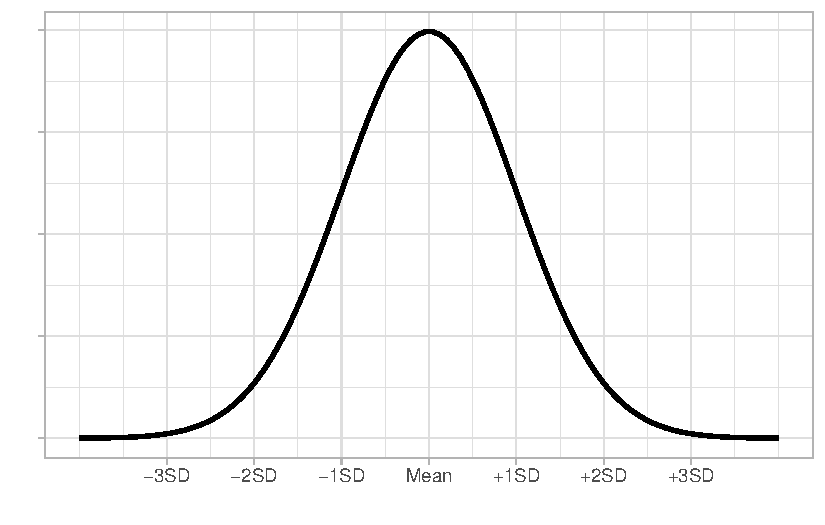
\includegraphics{combining_summarising_files/figure-pdf/normal distribution-1.pdf}

When data are normally distributed, the mean is the central peak of the
distribution. This is calculated by adding together all numbers in the
sample and dividing it by the sample size.

However, when the sample is not normally distributed and the peak does
not lie in the middle, extreme values or a longer tail will pull the
mean towards it. This means that where data are not normally
distributed, the mean will not be the centre and the value will be
invalid. Where this is the case, the \textbf{median} should be used
instead. The median is calculated by ordering the numeric values from
smallest to largest and selecting the middle value.

When data are normally distributed, the mean and median will give the
same, or very similar, values. This is because both are measuring the
centre. However, when the data are skewed, the mean and median will
differ. We prefer to use the mean where possible as it is the more
powerful measure. This means that it uses more of the data than the
median and is therefore more sensitive to changes in the sample.

\subsubsection{Measures of spread}\label{measures-of-spread}

Generally the measure of the spread of a numeric variable is presented
with a measure of spread, or how wide/narrow the distribution is. As
with the apread, the most appropriate values will depend on whether the
sample is normally distributed or not.

The most simple measure of spread is the \textbf{range} of a sample. In
R, this is given as two values: the minimum and the maximum.

The issue with using the range is that it is entirely defined by the
most extreme values in the sample and does not give any information
about the rest of it. An alternative to this would be to give the range
of the middle 50\%, also known as the \textbf{interquartile range}
(IQR).

The IQR is the difference between the 75th percentile, or upper
quartile, and the 25th percentile, or lower quartile. As with the
median, this is calculated by ordering the sample from smallest to
largest. The sample is then cut into 4 and the quartiles are calculated.
In R, the IQR is given as the difference between the upper and lower
quartiles. To calculate these values separately, we can use the
\texttt{quantile} function.

Both the range and IQR only use 2 values from the sample. As with the
median, these measures discard a lot of information from the summaries.
Where the sample is normally distributed, the \textbf{standard
deviation} (SD) can be used which measures the average distance between
each observation and the mean. The larger the SD, the wider and flatter
the normal curve will be; the smaller the SD, the narrower and taller
the curve will be:

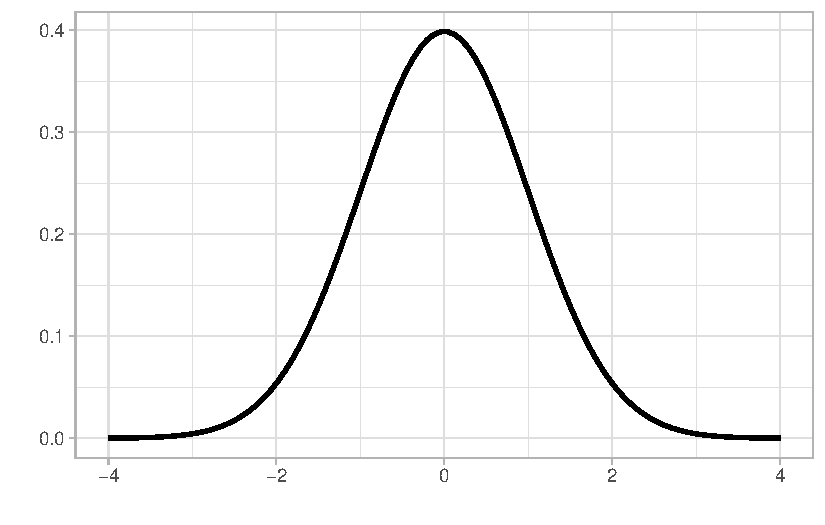
\includegraphics{combining_summarising_files/figure-pdf/normal distribution different sd-1.pdf}

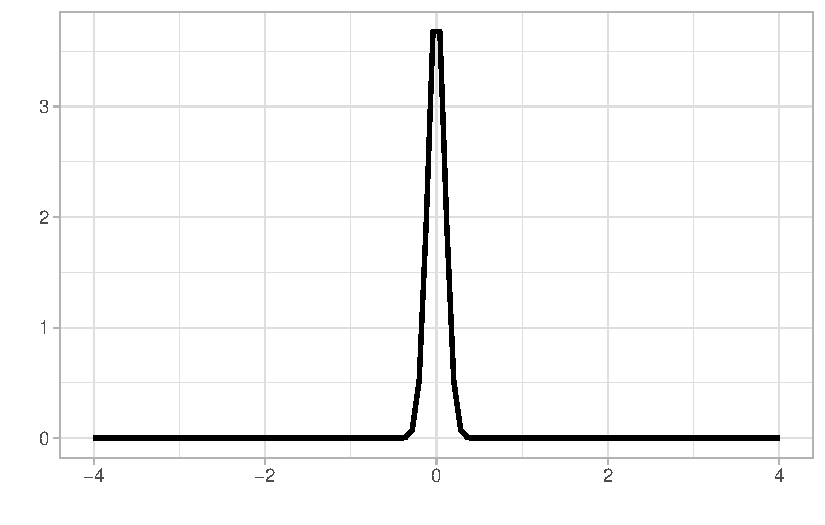
\includegraphics{combining_summarising_files/figure-pdf/normal distribution different sd-2.pdf}

The standard deviation is only appropriate where a numeric variable has
a normal distribution, otherwise this value is meaningless. If a sample
is normally distributed, then the entire sample can be completely
described just using the mean and standard deviation, even when the
sample values are not given. As the distribution is symmetrical, the
mean and standard deviation can be used to estimate ranges of values.
For example, it is known that approximately 68\% of a sample will lie
one standard deviation from the mean, approximately 95\% within 2
standard deviations from the mean, and around 99.7\% within 3 standard
deviations:

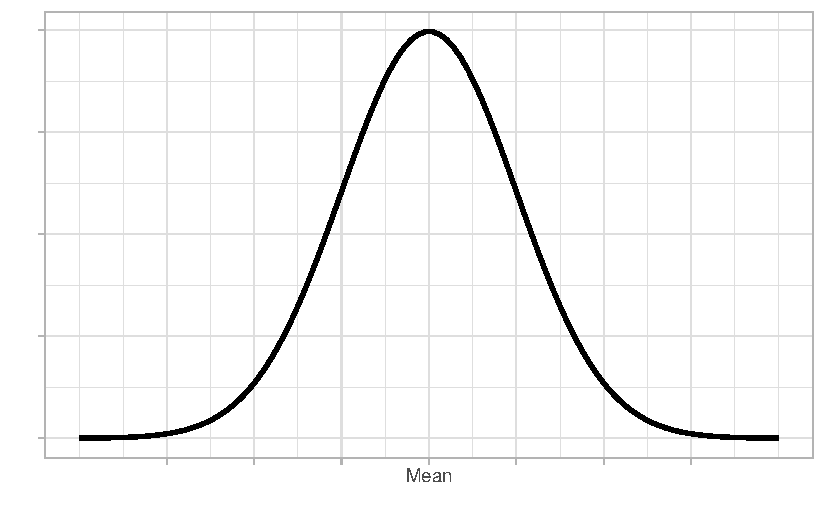
\includegraphics{combining_summarising_files/figure-pdf/normal with sd ranges-1.pdf}

This knowledge can also be used to check the mean and standard deviation
were appropriate summary statistics, even if we have no other
information.

\section{Exercise 4}\label{exercise-4}

\begin{enumerate}
\def\labelenumi{\arabic{enumi}.}
\item
  How many responders had both weekly rent and mortgage payments given?
  What are the potential reasons for this?
\item
  Combine the weekly rent and mortgage variables into a single weekly
  payment variable.
\item
  Create a summary table containing the mean, median, standard
  deviation, and the upper and lower quartiles of the weekly payment
  (rent and mortgage combined) for each region. What, if anything, can
  you infer about the distribution of this variable based on the table?
\end{enumerate}

\bookmarksetup{startatroot}

\chapter{Loading and tidying Excel
data}\label{loading-and-tidying-excel-data}

In the first part of the course, we saw how SPSS data (\texttt{.sav})
can be loaded into R using the \texttt{haven} package. Another common
format of data that cannot be loaded into base R is excel
(\texttt{.xlsx}). The package required to read Excel data is the
\texttt{readxl} package.

If this is the first time using the \texttt{readxl} package, remember to
install this to your machine using the \texttt{install.packages}
function:

\begin{Shaded}
\begin{Highlighting}[]
\FunctionTok{install.packages}\NormalTok{(}\StringTok{"readxl"}\NormalTok{)}
\end{Highlighting}
\end{Shaded}

Once this package has been installed, add it to the list of packages to
install at the top of your script file:

\begin{Shaded}
\begin{Highlighting}[]
\NormalTok{pacman}\SpecialCharTok{::}\FunctionTok{p\_load}\NormalTok{(tidyverse, haven, readxl)}
\end{Highlighting}
\end{Shaded}

\section{Loading an Excel sheet into
R}\label{loading-an-excel-sheet-into-r}

As with any file format, we must ensure data are in the correct form
before loading them into R, ensuring each column represents a variable,
each row represents an observation, and there are no tables or graphics.

Excel files can be a little tricker to manipulate than SPSS and CSV
files as they often contain multiple sheets. This is the case for the
data that we will be using for this part of the course.

The Excel file that we will be loading contains the
\href{https://view.officeapps.live.com/op/view.aspx?src=https\%3A\%2F\%2Fobr.uk\%2Fdocs\%2Fdlm_uploads\%2FDetailed_forecast_tables_Economy_March_2024.xlsx&wdOrigin=BROWSELINK}{Office
for Budget Responsibility (OBR) economic and fiscal outlook}. This
contains many sheets of data, but for this course we will just be
focusing on three:

\begin{itemize}
\tightlist
\item
  1.6 Labour market
\item
  1.14 National living wage
\item
  1.17 Housing market
\end{itemize}

Let's begin with housing market data, stored in the 18th sheet, labelled
``1.17''. This sheet can be selected in the \texttt{read\_xlsx} function
using the \texttt{sheet} argument.

The housing market sheet shows information over different time scales:
first by quarters, then years, and then across pairs of years. For this
example, we will extract information measured quarterly (rows 4 - 88).
The argument \texttt{range} allows us to define the range of cells (by
columns and rows) to extract.

Finally, we can see that the column headers are not in an appropriate
format for R: they contain spaces, brackets, and are very long! There
are two approaches we will consider to overcome this.

The first is to remove the column names completely (by not including
them in the \texttt{range} argument and setting
\texttt{col\_names\ =\ FALSE} within the \texttt{read\_xlsx} function)
and add them manually, using the \texttt{setNames} function.

Setting names manually can take a long time and a lot of typing if there
are many variables. An alternative to this manual approach is to include
them in the \texttt{range} of the \texttt{read\_xlsx} function, and use
an R function to `clean' them, making them follow the
\href{https://style.tidyverse.org/index.html}{style guide}.

\begin{tcolorbox}[enhanced jigsaw, bottomrule=.15mm, left=2mm, leftrule=.75mm, bottomtitle=1mm, coltitle=black, colbacktitle=quarto-callout-tip-color!10!white, toptitle=1mm, arc=.35mm, breakable, title=\textcolor{quarto-callout-tip-color}{\faLightbulb}\hspace{0.5em}{Style tip}, rightrule=.15mm, toprule=.15mm, opacityback=0, opacitybacktitle=0.6, titlerule=0mm, colback=white, colframe=quarto-callout-tip-color-frame]

The \texttt{janitor} package has been designed to format inputed data to
ensure it follows the Tidyverse style guide. The \texttt{clean\_names}
function can be applied to a data frame or tibble to adapt variable
names in this way.

\end{tcolorbox}

The following code loads the housing market sheet and manually sets the
variable names:

\begin{Shaded}
\begin{Highlighting}[]
\CommentTok{\# Return file names from the data folder}
\FunctionTok{list.files}\NormalTok{(}\AttributeTok{path =} \StringTok{"data"}\NormalTok{)}
\end{Highlighting}
\end{Shaded}

\begin{verbatim}
[1] "Detailed_forecast_tables_Economy_March_2024.xlsx"
[2] "generalfs21_EUL.sav"                             
[3] "interviewfs21_EUL.sav"                           
\end{verbatim}

\begin{Shaded}
\begin{Highlighting}[]
\NormalTok{housing\_market }\OtherTok{\textless{}{-}} 
  \FunctionTok{read\_xlsx}\NormalTok{(}\StringTok{"data/Detailed\_forecast\_tables\_Economy\_March\_2024.xlsx"}\NormalTok{,}
                            \CommentTok{\# Specify the sheet and range of cells to keep}
                            \AttributeTok{sheet =} \StringTok{"1.17"}\NormalTok{,}\AttributeTok{range =} \StringTok{"B4:J88"}\NormalTok{, }
                            \CommentTok{\# Remove column names (too messy)}
                            \AttributeTok{col\_names =} \ConstantTok{FALSE}\NormalTok{) }\SpecialCharTok{\%\textgreater{}\%} 
  \CommentTok{\# Add variable names manually}
  \FunctionTok{setNames}\NormalTok{(}\FunctionTok{c}\NormalTok{(}\StringTok{"period"}\NormalTok{, }\StringTok{"hpi\_comp15"}\NormalTok{, }\StringTok{"hpi\_prev\_year"}\NormalTok{, }
             \StringTok{"residential\_property\_transactions"}\NormalTok{, }
             \StringTok{"private\_enterprise\_housing\_starts"}\NormalTok{,}
             \StringTok{"private\_enterprise\_housing\_comp"}\NormalTok{, }
             \StringTok{"housing\_stock"}\NormalTok{, }\StringTok{"net\_additions\_housing\_stock"}\NormalTok{,}
             \StringTok{"turnover\_rate"}\NormalTok{))}
\end{Highlighting}
\end{Shaded}

The following code loads the same data but uses the \texttt{janitor}
package.

\begin{tcolorbox}[enhanced jigsaw, bottomrule=.15mm, left=2mm, leftrule=.75mm, bottomtitle=1mm, coltitle=black, colbacktitle=quarto-callout-warning-color!10!white, toptitle=1mm, arc=.35mm, breakable, title=\textcolor{quarto-callout-warning-color}{\faExclamationTriangle}\hspace{0.5em}{Warning}, rightrule=.15mm, toprule=.15mm, opacityback=0, opacitybacktitle=0.6, titlerule=0mm, colback=white, colframe=quarto-callout-warning-color-frame]

Do not run this code without installing and loading the \texttt{janitor}
package first. We will not run this during the course, but it is
included for future reference.

\end{tcolorbox}

\begin{Shaded}
\begin{Highlighting}[]
\NormalTok{housing\_market\_alt }\OtherTok{\textless{}{-}}
  \FunctionTok{read\_xlsx}\NormalTok{(}\StringTok{"data/Detailed\_forecast\_tables\_Economy\_March\_2024.xlsx"}\NormalTok{,}
                                \CommentTok{\# Specify the sheet and range of cells to keep}
                                \AttributeTok{sheet =} \StringTok{"1.17"}\NormalTok{,}\AttributeTok{range =} \StringTok{"B3:J88"}\NormalTok{) }\SpecialCharTok{\%\textgreater{}\%} 
  \CommentTok{\# Removes spaces, special characters, all lower case, etc.}
  \FunctionTok{clean\_names}\NormalTok{()}
\end{Highlighting}
\end{Shaded}

\section{Splitting variables}\label{splitting-variables}

In the current dataset, the time variable is given as a character and so
is not recognised as ordered or temporal by R. To overcome this, we can
split the variable to create separate year and quarter variables.

The \texttt{str\_sub} function from tidyverse's \texttt{stringr} package
extracts elements based on their position in a string of characters.
This can be used to return the first 4 digits to a new \texttt{year}
variable, and the final digit to a new \texttt{quarter} variable:

\begin{Shaded}
\begin{Highlighting}[]
\NormalTok{housing\_market }\OtherTok{\textless{}{-}}\NormalTok{ housing\_market }\SpecialCharTok{\%\textgreater{}\%}
  \CommentTok{\# Don\textquotesingle{}t forget to convert the string to numberic}
  \FunctionTok{mutate}\NormalTok{(}\AttributeTok{year =}  \FunctionTok{as.numeric}\NormalTok{(}\FunctionTok{str\_sub}\NormalTok{(period, }\AttributeTok{start =} \DecValTok{1}\NormalTok{, }\AttributeTok{end =} \DecValTok{4}\NormalTok{)),}
         \AttributeTok{quarter =} \FunctionTok{as.numeric}\NormalTok{(}\FunctionTok{str\_sub}\NormalTok{(period, }
                              \CommentTok{\# Use {-} to work from the end of the string}
                              \AttributeTok{start =} \SpecialCharTok{{-}}\DecValTok{1}\NormalTok{L, }\AttributeTok{end =} \SpecialCharTok{{-}}\DecValTok{1}\NormalTok{L))) }\SpecialCharTok{\%\textgreater{}\%} 
  \CommentTok{\# Remove the original period variable}
  \FunctionTok{select}\NormalTok{(}\SpecialCharTok{{-}}\NormalTok{period)}
\end{Highlighting}
\end{Shaded}

\section{Exercise 5}\label{exercise-5}

\begin{enumerate}
\def\labelenumi{\arabic{enumi}.}
\tightlist
\item
  Load in the OBR's quarterly labour market data (sheet 1.6), keeping
  the following variables:
\end{enumerate}

\begin{itemize}
\tightlist
\item
  Period
\item
  Employment rate (\%)
\item
  Average earning growth (\%)
\item
  Average earning index
\item
  Productivity per hour index
\item
  Real wage product
\item
  Real consumption wage
\end{itemize}

Split the period data into separate year and quarter variables, ensure
that all variable names follow Tidyverse's style guide. Name this object
\texttt{labour\_market}.

\begin{enumerate}
\def\labelenumi{\arabic{enumi}.}
\setcounter{enumi}{1}
\tightlist
\item
  Load the OBR's national living wage data (sheet 1.14), keep as an
  object named \texttt{living\_wage}.
\end{enumerate}

\section{Tranforming data}\label{tranforming-data}

The labour market and housing market data are currently considered in
what is known as \textbf{long format}, with many rows and fewer
variables. The alternative to this format, \textbf{wide format}, can be
seen in the living wage data, which has many variables and very few
(only one!) row. Sometimes we may wish to convert between these
variables, either to join them to other datasets (as is the case here),
or to carry out an analysis or visualisation that requires a certain
format. These conversions are carried out using the
\texttt{pivot\_longer} or \texttt{pivot\_wider} functions.

There are many ways to pivot data within R (see the helpfile
\texttt{?pivot\_longer} for a full list of arguments), and the setup of
this function tends to differ for every situation. For worked examples
and a more detailed explanation of the function's capabilities, enter
\texttt{vignette("pivot")} into the console. For our data, we will need
to convert the wide-format living wage data to a long-format so we are
able to join it to the other data. This will create a new dataset with 2
variables: year and living wage, with a row per year. The \texttt{year}
variable will be taken from the wide data names, and the
\texttt{living\_wage} variable will come from the wide data values:

\begin{Shaded}
\begin{Highlighting}[]
\NormalTok{living\_wage\_long }\OtherTok{\textless{}{-}}\NormalTok{ living\_wage }\SpecialCharTok{\%\textgreater{}\%} 
  \CommentTok{\# First, select the columns that we wish to pivot (all of them)}
  \FunctionTok{pivot\_longer}\NormalTok{(}\AttributeTok{cols =} \FunctionTok{everything}\NormalTok{(),}
               \CommentTok{\# Move the old variable names to a new year variable}
               \AttributeTok{names\_to =} \StringTok{"year"}\NormalTok{,}
               \CommentTok{\# Remove the prefix from the old variable names}
               \AttributeTok{names\_prefix =} \StringTok{"year\_"}\NormalTok{,}
               \CommentTok{\# Convert the new year variable to numeric}
               \AttributeTok{names\_transform =}\NormalTok{ as.numeric,}
               \CommentTok{\# Take the old values and create a new living\_wage variable}
               \AttributeTok{values\_to =} \StringTok{"living\_wage"}\NormalTok{)}
\end{Highlighting}
\end{Shaded}

\section{Exercise 6}\label{exercise-6}

\begin{enumerate}
\def\labelenumi{\arabic{enumi}.}
\tightlist
\item
  Combine all three OBR datasets (housing market, labour market and
  living wage) together to create one complete dataset,
  \texttt{obr\_data}.
\end{enumerate}

\bookmarksetup{startatroot}

\chapter{Data visualisation}\label{data-visualisation}

Data visualisation is a powerful tool with many important uses. First,
visualisations allow us to explore the data, identify potential outliers
and errors, or check that the variables behave in the way we would
expect them to if they had been recorded correctly. Visualisations can
also be used as an analysis tool, allowing us to identify trends in the
data or differences between groups. Finally, visualisations can help to
convey messages to an audience in a clear, concise way that is often
more powerful than presenting them using numbers or text. In some cases,
data visualisations can show results so clearly that further analysis is
arguably unnecessary.

\section{Choosing the most appropriate
visualisation}\label{choosing-the-most-appropriate-visualisation}

The most appropriate choice of visualisation will depend on the type of
variable(s) we wish to display, the number of variables and the message
we are trying to disseminate. Common plots used to display combinations
of different types of data are given in following table:

\global\setlength{\Oldarrayrulewidth}{\arrayrulewidth}

\global\setlength{\Oldtabcolsep}{\tabcolsep}

\setlength{\tabcolsep}{2pt}

\renewcommand*{\arraystretch}{1.5}



\providecommand{\ascline}[3]{\noalign{\global\arrayrulewidth #1}\arrayrulecolor[HTML]{#2}\cline{#3}}

\begin{longtable*}[c]{|p{1.65in}|p{2.30in}|p{3.45in}|p{2.13in}}



\hhline{>{\arrayrulecolor[HTML]{666666}\global\arrayrulewidth=1.5pt}->{\arrayrulecolor[HTML]{666666}\global\arrayrulewidth=1.5pt}->{\arrayrulecolor[HTML]{666666}\global\arrayrulewidth=1.5pt}->{\arrayrulecolor[HTML]{666666}\global\arrayrulewidth=1.5pt}-}

\multicolumn{1}{>{\raggedright}m{\dimexpr 1.65in+0\tabcolsep}}{\textcolor[HTML]{000000}{\fontsize{11}{11}\selectfont{\global\setmainfont{Arial}{\textbf{Number\ of\ variables}}}}} & \multicolumn{1}{!{\color[HTML]{666666}\vrule width 1pt}>{\raggedright}m{\dimexpr 2.3in+0\tabcolsep}}{\textcolor[HTML]{000000}{\fontsize{11}{11}\selectfont{\global\setmainfont{Arial}{\textbf{Type\ of\ variables}}}}} & \multicolumn{1}{!{\color[HTML]{666666}\vrule width 1pt}>{\raggedright}m{\dimexpr 3.45in+0\tabcolsep}}{\textcolor[HTML]{000000}{\fontsize{11}{11}\selectfont{\global\setmainfont{Arial}{\textbf{Visualisation}}}}} & \multicolumn{1}{!{\color[HTML]{666666}\vrule width 1pt}>{\raggedright}m{\dimexpr 2.13in+0\tabcolsep}}{\textcolor[HTML]{000000}{\fontsize{11}{11}\selectfont{\global\setmainfont{Arial}{\textbf{geom\ object\ (or\ R\ function)}}}}} \\

\noalign{\global\arrayrulewidth 0pt}\arrayrulecolor[HTML]{000000}

\hhline{>{\arrayrulecolor[HTML]{666666}\global\arrayrulewidth=1.5pt}-|>{\arrayrulecolor[HTML]{666666}\global\arrayrulewidth=1.5pt}-|>{\arrayrulecolor[HTML]{666666}\global\arrayrulewidth=1.5pt}-|>{\arrayrulecolor[HTML]{666666}\global\arrayrulewidth=1.5pt}-}\endfirsthead 

\hhline{>{\arrayrulecolor[HTML]{666666}\global\arrayrulewidth=1.5pt}->{\arrayrulecolor[HTML]{666666}\global\arrayrulewidth=1.5pt}->{\arrayrulecolor[HTML]{666666}\global\arrayrulewidth=1.5pt}->{\arrayrulecolor[HTML]{666666}\global\arrayrulewidth=1.5pt}-}

\multicolumn{1}{>{\raggedright}m{\dimexpr 1.65in+0\tabcolsep}}{\textcolor[HTML]{000000}{\fontsize{11}{11}\selectfont{\global\setmainfont{Arial}{\textbf{Number\ of\ variables}}}}} & \multicolumn{1}{!{\color[HTML]{666666}\vrule width 1pt}>{\raggedright}m{\dimexpr 2.3in+0\tabcolsep}}{\textcolor[HTML]{000000}{\fontsize{11}{11}\selectfont{\global\setmainfont{Arial}{\textbf{Type\ of\ variables}}}}} & \multicolumn{1}{!{\color[HTML]{666666}\vrule width 1pt}>{\raggedright}m{\dimexpr 3.45in+0\tabcolsep}}{\textcolor[HTML]{000000}{\fontsize{11}{11}\selectfont{\global\setmainfont{Arial}{\textbf{Visualisation}}}}} & \multicolumn{1}{!{\color[HTML]{666666}\vrule width 1pt}>{\raggedright}m{\dimexpr 2.13in+0\tabcolsep}}{\textcolor[HTML]{000000}{\fontsize{11}{11}\selectfont{\global\setmainfont{Arial}{\textbf{geom\ object\ (or\ R\ function)}}}}} \\

\noalign{\global\arrayrulewidth 0pt}\arrayrulecolor[HTML]{000000}

\hhline{>{\arrayrulecolor[HTML]{666666}\global\arrayrulewidth=1.5pt}-|>{\arrayrulecolor[HTML]{666666}\global\arrayrulewidth=1.5pt}-|>{\arrayrulecolor[HTML]{666666}\global\arrayrulewidth=1.5pt}-|>{\arrayrulecolor[HTML]{666666}\global\arrayrulewidth=1.5pt}-}\endhead



\multicolumn{1}{>{\cellcolor[HTML]{F2F2F2}\raggedright}m{\dimexpr 1.65in+0\tabcolsep}}{} & \multicolumn{1}{!{\color[HTML]{666666}\vrule width 1pt}>{\cellcolor[HTML]{F2F2F2}\raggedright}m{\dimexpr 2.3in+0\tabcolsep}}{} & \multicolumn{1}{!{\color[HTML]{666666}\vrule width 1pt}>{\cellcolor[HTML]{F2F2F2}\raggedright}m{\dimexpr 3.45in+0\tabcolsep}}{\textcolor[HTML]{000000}{\fontsize{11}{11}\selectfont{\global\setmainfont{Arial}{Frequency\ table}}}} & \multicolumn{1}{!{\color[HTML]{666666}\vrule width 1pt}>{\cellcolor[HTML]{F2F2F2}\raggedright}m{\dimexpr 2.13in+0\tabcolsep}}{\textcolor[HTML]{000000}{\fontsize{11}{11}\selectfont{\global\setmainfont{Arial}{table}}}} \\

\noalign{\global\arrayrulewidth 0pt}\arrayrulecolor[HTML]{000000}

\hhline{>{\arrayrulecolor[HTML]{000000}\global\arrayrulewidth=0pt}->{\arrayrulecolor[HTML]{000000}\global\arrayrulewidth=0pt}->{\arrayrulecolor[HTML]{666666}\global\arrayrulewidth=1pt}-|>{\arrayrulecolor[HTML]{666666}\global\arrayrulewidth=1pt}-}



\multicolumn{1}{>{\cellcolor[HTML]{F2F2F2}\raggedright}m{\dimexpr 1.65in+0\tabcolsep}}{} & \multicolumn{1}{!{\color[HTML]{666666}\vrule width 1pt}>{\cellcolor[HTML]{F2F2F2}\raggedright}m{\dimexpr 2.3in+0\tabcolsep}}{\multirow[c]{-2}{*}{\parbox{2.3in}{\raggedright \textcolor[HTML]{000000}{\fontsize{11}{11}\selectfont{\global\setmainfont{Arial}{Categorical}}}}}} & \multicolumn{1}{!{\color[HTML]{666666}\vrule width 1pt}>{\cellcolor[HTML]{F2F2F2}\raggedright}m{\dimexpr 3.45in+0\tabcolsep}}{\textcolor[HTML]{000000}{\fontsize{11}{11}\selectfont{\global\setmainfont{Arial}{Bar\ chart}}}} & \multicolumn{1}{!{\color[HTML]{666666}\vrule width 1pt}>{\cellcolor[HTML]{F2F2F2}\raggedright}m{\dimexpr 2.13in+0\tabcolsep}}{\textcolor[HTML]{000000}{\fontsize{11}{11}\selectfont{\global\setmainfont{Arial}{geom\_bar}}}} \\

\noalign{\global\arrayrulewidth 0pt}\arrayrulecolor[HTML]{000000}

\hhline{>{\arrayrulecolor[HTML]{000000}\global\arrayrulewidth=0pt}->{\arrayrulecolor[HTML]{666666}\global\arrayrulewidth=1pt}-|>{\arrayrulecolor[HTML]{666666}\global\arrayrulewidth=1pt}-|>{\arrayrulecolor[HTML]{666666}\global\arrayrulewidth=1pt}-}



\multicolumn{1}{>{\cellcolor[HTML]{F2F2F2}\raggedright}m{\dimexpr 1.65in+0\tabcolsep}}{} & \multicolumn{1}{!{\color[HTML]{666666}\vrule width 1pt}>{\cellcolor[HTML]{F2F2F2}\raggedright}m{\dimexpr 2.3in+0\tabcolsep}}{\textcolor[HTML]{000000}{\fontsize{11}{11}\selectfont{\global\setmainfont{Arial}{Numerical}}}} & \multicolumn{1}{!{\color[HTML]{666666}\vrule width 1pt}>{\cellcolor[HTML]{F2F2F2}\raggedright}m{\dimexpr 3.45in+0\tabcolsep}}{\textcolor[HTML]{000000}{\fontsize{11}{11}\selectfont{\global\setmainfont{Arial}{Histogram}}}} & \multicolumn{1}{!{\color[HTML]{666666}\vrule width 1pt}>{\cellcolor[HTML]{F2F2F2}\raggedright}m{\dimexpr 2.13in+0\tabcolsep}}{\textcolor[HTML]{000000}{\fontsize{11}{11}\selectfont{\global\setmainfont{Arial}{geom\_histogram}}}} \\

\noalign{\global\arrayrulewidth 0pt}\arrayrulecolor[HTML]{000000}

\hhline{>{\arrayrulecolor[HTML]{000000}\global\arrayrulewidth=0pt}->{\arrayrulecolor[HTML]{666666}\global\arrayrulewidth=1pt}-|>{\arrayrulecolor[HTML]{666666}\global\arrayrulewidth=1pt}-|>{\arrayrulecolor[HTML]{666666}\global\arrayrulewidth=1pt}-}



\multicolumn{1}{>{\cellcolor[HTML]{F2F2F2}\raggedright}m{\dimexpr 1.65in+0\tabcolsep}}{} & \multicolumn{1}{!{\color[HTML]{666666}\vrule width 1pt}>{\cellcolor[HTML]{F2F2F2}\raggedright}m{\dimexpr 2.3in+0\tabcolsep}}{\textcolor[HTML]{000000}{\fontsize{11}{11}\selectfont{\global\setmainfont{Arial}{Spatial}}}} & \multicolumn{1}{!{\color[HTML]{666666}\vrule width 1pt}>{\cellcolor[HTML]{F2F2F2}\raggedright}m{\dimexpr 3.45in+0\tabcolsep}}{\textcolor[HTML]{000000}{\fontsize{11}{11}\selectfont{\global\setmainfont{Arial}{Map}}}} & \multicolumn{1}{!{\color[HTML]{666666}\vrule width 1pt}>{\cellcolor[HTML]{F2F2F2}\raggedright}m{\dimexpr 2.13in+0\tabcolsep}}{\textcolor[HTML]{000000}{\fontsize{11}{11}\selectfont{\global\setmainfont{Arial}{geom\_sf}}}} \\

\noalign{\global\arrayrulewidth 0pt}\arrayrulecolor[HTML]{000000}

\hhline{>{\arrayrulecolor[HTML]{000000}\global\arrayrulewidth=0pt}->{\arrayrulecolor[HTML]{666666}\global\arrayrulewidth=1pt}-|>{\arrayrulecolor[HTML]{666666}\global\arrayrulewidth=1pt}-|>{\arrayrulecolor[HTML]{666666}\global\arrayrulewidth=1pt}-}



\multicolumn{1}{>{\cellcolor[HTML]{F2F2F2}\raggedright}m{\dimexpr 1.65in+0\tabcolsep}}{\multirow[c]{-5}{*}{\parbox{1.65in}{\raggedright \textcolor[HTML]{000000}{\fontsize{11}{11}\selectfont{\global\setmainfont{Arial}{One\ variable}}}}}} & \multicolumn{1}{!{\color[HTML]{666666}\vrule width 1pt}>{\cellcolor[HTML]{F2F2F2}\raggedright}m{\dimexpr 2.3in+0\tabcolsep}}{\textcolor[HTML]{000000}{\fontsize{11}{11}\selectfont{\global\setmainfont{Arial}{Temporal}}}} & \multicolumn{1}{!{\color[HTML]{666666}\vrule width 1pt}>{\cellcolor[HTML]{F2F2F2}\raggedright}m{\dimexpr 3.45in+0\tabcolsep}}{\textcolor[HTML]{000000}{\fontsize{11}{11}\selectfont{\global\setmainfont{Arial}{Line\ plot}}}} & \multicolumn{1}{!{\color[HTML]{666666}\vrule width 1pt}>{\cellcolor[HTML]{F2F2F2}\raggedright}m{\dimexpr 2.13in+0\tabcolsep}}{\textcolor[HTML]{000000}{\fontsize{11}{11}\selectfont{\global\setmainfont{Arial}{geom\_line}}}} \\

\noalign{\global\arrayrulewidth 0pt}\arrayrulecolor[HTML]{000000}

\hhline{>{\arrayrulecolor[HTML]{666666}\global\arrayrulewidth=1pt}-|>{\arrayrulecolor[HTML]{666666}\global\arrayrulewidth=1pt}-|>{\arrayrulecolor[HTML]{666666}\global\arrayrulewidth=1pt}-|>{\arrayrulecolor[HTML]{666666}\global\arrayrulewidth=1pt}-}



\multicolumn{1}{>{\cellcolor[HTML]{F2F2F2}\raggedright}m{\dimexpr 1.65in+0\tabcolsep}}{} & \multicolumn{1}{!{\color[HTML]{666666}\vrule width 1pt}>{\cellcolor[HTML]{F2F2F2}\raggedright}m{\dimexpr 2.3in+0\tabcolsep}}{} & \multicolumn{1}{!{\color[HTML]{666666}\vrule width 1pt}>{\cellcolor[HTML]{F2F2F2}\raggedright}m{\dimexpr 3.45in+0\tabcolsep}}{\textcolor[HTML]{000000}{\fontsize{11}{11}\selectfont{\global\setmainfont{Arial}{Frequency\ table}}}} & \multicolumn{1}{!{\color[HTML]{666666}\vrule width 1pt}>{\cellcolor[HTML]{F2F2F2}\raggedright}m{\dimexpr 2.13in+0\tabcolsep}}{\textcolor[HTML]{000000}{\fontsize{11}{11}\selectfont{\global\setmainfont{Arial}{table}}}} \\

\noalign{\global\arrayrulewidth 0pt}\arrayrulecolor[HTML]{000000}

\hhline{>{\arrayrulecolor[HTML]{000000}\global\arrayrulewidth=0pt}->{\arrayrulecolor[HTML]{000000}\global\arrayrulewidth=0pt}->{\arrayrulecolor[HTML]{666666}\global\arrayrulewidth=1pt}-|>{\arrayrulecolor[HTML]{666666}\global\arrayrulewidth=1pt}-}



\multicolumn{1}{>{\cellcolor[HTML]{F2F2F2}\raggedright}m{\dimexpr 1.65in+0\tabcolsep}}{} & \multicolumn{1}{!{\color[HTML]{666666}\vrule width 1pt}>{\cellcolor[HTML]{F2F2F2}\raggedright}m{\dimexpr 2.3in+0\tabcolsep}}{\multirow[c]{-2}{*}{\parbox{2.3in}{\raggedright \textcolor[HTML]{000000}{\fontsize{11}{11}\selectfont{\global\setmainfont{Arial}{Two\ categorical}}}}}} & \multicolumn{1}{!{\color[HTML]{666666}\vrule width 1pt}>{\cellcolor[HTML]{F2F2F2}\raggedright}m{\dimexpr 3.45in+0\tabcolsep}}{\textcolor[HTML]{000000}{\fontsize{11}{11}\selectfont{\global\setmainfont{Arial}{Stacked/side-by-side\ bar\ chart}}}} & \multicolumn{1}{!{\color[HTML]{666666}\vrule width 1pt}>{\cellcolor[HTML]{F2F2F2}\raggedright}m{\dimexpr 2.13in+0\tabcolsep}}{\textcolor[HTML]{000000}{\fontsize{11}{11}\selectfont{\global\setmainfont{Arial}{geom\_bar}}}} \\

\noalign{\global\arrayrulewidth 0pt}\arrayrulecolor[HTML]{000000}

\hhline{>{\arrayrulecolor[HTML]{000000}\global\arrayrulewidth=0pt}->{\arrayrulecolor[HTML]{666666}\global\arrayrulewidth=1pt}-|>{\arrayrulecolor[HTML]{666666}\global\arrayrulewidth=1pt}-|>{\arrayrulecolor[HTML]{666666}\global\arrayrulewidth=1pt}-}



\multicolumn{1}{>{\cellcolor[HTML]{F2F2F2}\raggedright}m{\dimexpr 1.65in+0\tabcolsep}}{} & \multicolumn{1}{!{\color[HTML]{666666}\vrule width 1pt}>{\cellcolor[HTML]{F2F2F2}\raggedright}m{\dimexpr 2.3in+0\tabcolsep}}{} & \multicolumn{1}{!{\color[HTML]{666666}\vrule width 1pt}>{\cellcolor[HTML]{F2F2F2}\raggedright}m{\dimexpr 3.45in+0\tabcolsep}}{\textcolor[HTML]{000000}{\fontsize{11}{11}\selectfont{\global\setmainfont{Arial}{Dot\ plot}}}} & \multicolumn{1}{!{\color[HTML]{666666}\vrule width 1pt}>{\cellcolor[HTML]{F2F2F2}\raggedright}m{\dimexpr 2.13in+0\tabcolsep}}{\textcolor[HTML]{000000}{\fontsize{11}{11}\selectfont{\global\setmainfont{Arial}{geom\_point}}}} \\

\noalign{\global\arrayrulewidth 0pt}\arrayrulecolor[HTML]{000000}

\hhline{>{\arrayrulecolor[HTML]{000000}\global\arrayrulewidth=0pt}->{\arrayrulecolor[HTML]{000000}\global\arrayrulewidth=0pt}->{\arrayrulecolor[HTML]{666666}\global\arrayrulewidth=1pt}-|>{\arrayrulecolor[HTML]{666666}\global\arrayrulewidth=1pt}-}



\multicolumn{1}{>{\cellcolor[HTML]{F2F2F2}\raggedright}m{\dimexpr 1.65in+0\tabcolsep}}{} & \multicolumn{1}{!{\color[HTML]{666666}\vrule width 1pt}>{\cellcolor[HTML]{F2F2F2}\raggedright}m{\dimexpr 2.3in+0\tabcolsep}}{\multirow[c]{-2}{*}{\parbox{2.3in}{\raggedright \textcolor[HTML]{000000}{\fontsize{11}{11}\selectfont{\global\setmainfont{Arial}{One\ numeric,\ one\ categorical}}}}}} & \multicolumn{1}{!{\color[HTML]{666666}\vrule width 1pt}>{\cellcolor[HTML]{F2F2F2}\raggedright}m{\dimexpr 3.45in+0\tabcolsep}}{\textcolor[HTML]{000000}{\fontsize{11}{11}\selectfont{\global\setmainfont{Arial}{Box\ plot}}}} & \multicolumn{1}{!{\color[HTML]{666666}\vrule width 1pt}>{\cellcolor[HTML]{F2F2F2}\raggedright}m{\dimexpr 2.13in+0\tabcolsep}}{\textcolor[HTML]{000000}{\fontsize{11}{11}\selectfont{\global\setmainfont{Arial}{geom\_boxplot}}}} \\

\noalign{\global\arrayrulewidth 0pt}\arrayrulecolor[HTML]{000000}

\hhline{>{\arrayrulecolor[HTML]{000000}\global\arrayrulewidth=0pt}->{\arrayrulecolor[HTML]{666666}\global\arrayrulewidth=1pt}-|>{\arrayrulecolor[HTML]{666666}\global\arrayrulewidth=1pt}-|>{\arrayrulecolor[HTML]{666666}\global\arrayrulewidth=1pt}-}



\multicolumn{1}{>{\cellcolor[HTML]{F2F2F2}\raggedright}m{\dimexpr 1.65in+0\tabcolsep}}{\multirow[c]{-5}{*}{\parbox{1.65in}{\raggedright \textcolor[HTML]{000000}{\fontsize{11}{11}\selectfont{\global\setmainfont{Arial}{Two\ variables}}}}}} & \multicolumn{1}{!{\color[HTML]{666666}\vrule width 1pt}>{\cellcolor[HTML]{F2F2F2}\raggedright}m{\dimexpr 2.3in+0\tabcolsep}}{\textcolor[HTML]{000000}{\fontsize{11}{11}\selectfont{\global\setmainfont{Arial}{Two\ numerical}}}} & \multicolumn{1}{!{\color[HTML]{666666}\vrule width 1pt}>{\cellcolor[HTML]{F2F2F2}\raggedright}m{\dimexpr 3.45in+0\tabcolsep}}{\textcolor[HTML]{000000}{\fontsize{11}{11}\selectfont{\global\setmainfont{Arial}{Scatterplot}}}} & \multicolumn{1}{!{\color[HTML]{666666}\vrule width 1pt}>{\cellcolor[HTML]{F2F2F2}\raggedright}m{\dimexpr 2.13in+0\tabcolsep}}{\textcolor[HTML]{000000}{\fontsize{11}{11}\selectfont{\global\setmainfont{Arial}{geom\_point}}}} \\

\noalign{\global\arrayrulewidth 0pt}\arrayrulecolor[HTML]{000000}

\hhline{>{\arrayrulecolor[HTML]{666666}\global\arrayrulewidth=1pt}-|>{\arrayrulecolor[HTML]{666666}\global\arrayrulewidth=1pt}-|>{\arrayrulecolor[HTML]{666666}\global\arrayrulewidth=1pt}-|>{\arrayrulecolor[HTML]{666666}\global\arrayrulewidth=1pt}-}



\multicolumn{1}{>{\cellcolor[HTML]{F2F2F2}\raggedright}m{\dimexpr 1.65in+0\tabcolsep}}{} & \multicolumn{1}{!{\color[HTML]{666666}\vrule width 1pt}>{\cellcolor[HTML]{F2F2F2}\raggedright}m{\dimexpr 2.3in+0\tabcolsep}}{\textcolor[HTML]{000000}{\fontsize{11}{11}\selectfont{\global\setmainfont{Arial}{>\ 2\ categorical}}}} & \multicolumn{1}{!{\color[HTML]{666666}\vrule width 1pt}>{\cellcolor[HTML]{F2F2F2}\raggedright}m{\dimexpr 3.45in+0\tabcolsep}}{\textcolor[HTML]{000000}{\fontsize{11}{11}\selectfont{\global\setmainfont{Arial}{Table}}}} & \multicolumn{1}{!{\color[HTML]{666666}\vrule width 1pt}>{\cellcolor[HTML]{F2F2F2}\raggedright}m{\dimexpr 2.13in+0\tabcolsep}}{\textcolor[HTML]{000000}{\fontsize{11}{11}\selectfont{\global\setmainfont{Arial}{table}}}} \\

\noalign{\global\arrayrulewidth 0pt}\arrayrulecolor[HTML]{000000}

\hhline{>{\arrayrulecolor[HTML]{000000}\global\arrayrulewidth=0pt}->{\arrayrulecolor[HTML]{666666}\global\arrayrulewidth=1pt}-|>{\arrayrulecolor[HTML]{666666}\global\arrayrulewidth=1pt}-|>{\arrayrulecolor[HTML]{666666}\global\arrayrulewidth=1pt}-}



\multicolumn{1}{>{\cellcolor[HTML]{F2F2F2}\raggedright}m{\dimexpr 1.65in+0\tabcolsep}}{\multirow[c]{-2}{*}{\parbox{1.65in}{\raggedright \textcolor[HTML]{000000}{\fontsize{11}{11}\selectfont{\global\setmainfont{Arial}{>\ 2\ variables}}}}}} & \multicolumn{1}{!{\color[HTML]{666666}\vrule width 1pt}>{\cellcolor[HTML]{F2F2F2}\raggedright}m{\dimexpr 2.3in+0\tabcolsep}}{\textcolor[HTML]{000000}{\fontsize{11}{11}\selectfont{\global\setmainfont{Arial}{2\ numeric,\ one\ categorical\ or\ }}}\textcolor[HTML]{000000}{\fontsize{11}{11}\selectfont{\global\setmainfont{Arial}{\linebreak }}}\textcolor[HTML]{000000}{\fontsize{11}{11}\selectfont{\global\setmainfont{Arial}{>\ 2\ numeric}}}} & \multicolumn{1}{!{\color[HTML]{666666}\vrule width 1pt}>{\cellcolor[HTML]{F2F2F2}\raggedright}m{\dimexpr 3.45in+0\tabcolsep}}{\textcolor[HTML]{000000}{\fontsize{11}{11}\selectfont{\global\setmainfont{Arial}{Scatterplot\ with\ different\ colours/symbols/sizes}}}} & \multicolumn{1}{!{\color[HTML]{666666}\vrule width 1pt}>{\cellcolor[HTML]{F2F2F2}\raggedright}m{\dimexpr 2.13in+0\tabcolsep}}{\textcolor[HTML]{000000}{\fontsize{11}{11}\selectfont{\global\setmainfont{Arial}{geom\_point}}}} \\

\noalign{\global\arrayrulewidth 0pt}\arrayrulecolor[HTML]{000000}

\hhline{>{\arrayrulecolor[HTML]{666666}\global\arrayrulewidth=1pt}-|>{\arrayrulecolor[HTML]{666666}\global\arrayrulewidth=1pt}-|>{\arrayrulecolor[HTML]{666666}\global\arrayrulewidth=1pt}-|>{\arrayrulecolor[HTML]{666666}\global\arrayrulewidth=1pt}-}



\end{longtable*}



\arrayrulecolor[HTML]{000000}

\global\setlength{\arrayrulewidth}{\Oldarrayrulewidth}

\global\setlength{\tabcolsep}{\Oldtabcolsep}

\renewcommand*{\arraystretch}{1}

R is very flexible when it comes to visualising data and contains a wide
variety of options to customise graphs. This section will focus on the
Tidyverse package \texttt{ggplot2} and introduce some of the more
commonly used graphical functions and parameters.

\section{The ggplot2 package}\label{the-ggplot2-package}

The \texttt{ggplot2} package implements the `grammar of graphics', a
system that aims to describe all statistical graphics in terms of their
components or layers. All graphics can be broken down into the same
components: the data, a coordinate system (or plot area) and some visual
markings of the data. More complex plots may have additional layers but
all must contain these three.

For example, if we want to investigate the distribution of tenure types
between responses of the English Housing Survey (EHS), we could use a
\textbf{bar chart}. The visual markings for a bar chart is a bar per
group (in this case, tenure type), where the length of each bar
represents the number of observations within that group.

For any visualisation created using \texttt{ggplot2}, we first use the
\texttt{ggplot} function to create a coordinate system (a blank plot
space) that we can add layers and objects to. Within this function, we
specify the data that we wish to display on the coordinate system:

\begin{Shaded}
\begin{Highlighting}[]
\FunctionTok{ggplot}\NormalTok{(}\AttributeTok{data =}\NormalTok{ ehs\_tidy)}
\end{Highlighting}
\end{Shaded}

To add information to this graph, we add a \textbf{geom} layer: a visual
representation of the data. There are many different geom objects built
into the ggplot2 package (begin typing \texttt{?geom} into the console
to see a list). The \texttt{geom\_bar} function is used to create bar
charts

Each geom object must contain a mapping argument, coupled with the
\texttt{aes} function which defines how the variables in the dataset are
visualised. In this case, we use the \texttt{aes} function to specify
the grouping variable on the x axis, but it can also be used to set the
colour, size or symbol based on variable values.

\begin{tcolorbox}[enhanced jigsaw, bottomrule=.15mm, left=2mm, leftrule=.75mm, bottomtitle=1mm, coltitle=black, colbacktitle=quarto-callout-warning-color!10!white, toptitle=1mm, arc=.35mm, breakable, title=\textcolor{quarto-callout-warning-color}{\faExclamationTriangle}\hspace{0.5em}{Warning}, rightrule=.15mm, toprule=.15mm, opacityback=0, opacitybacktitle=0.6, titlerule=0mm, colback=white, colframe=quarto-callout-warning-color-frame]

Although \texttt{ggplot2} is part of the tidverse package, it uses a
\texttt{+} symbol to add layers to visualisations rather than the pipe
\texttt{\%\textgreater{}\%} we have been using in other packages.

\end{tcolorbox}

\begin{Shaded}
\begin{Highlighting}[]
\FunctionTok{ggplot}\NormalTok{(}\AttributeTok{data =}\NormalTok{ ehs\_tidy) }\SpecialCharTok{+}
  \FunctionTok{geom\_bar}\NormalTok{(}\AttributeTok{mapping =} \FunctionTok{aes}\NormalTok{(}\AttributeTok{x =}\NormalTok{ tenure\_type))}
\end{Highlighting}
\end{Shaded}

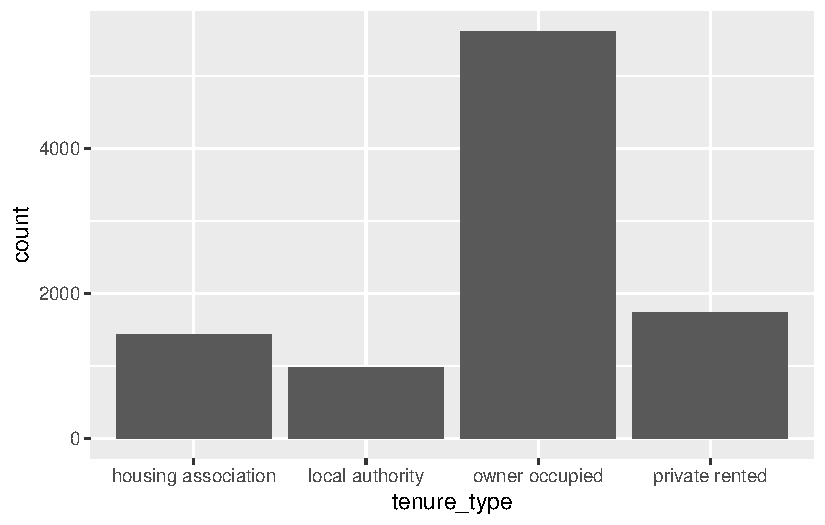
\includegraphics{visualisation_files/figure-pdf/bar chart tenure_type-1.pdf}

Graphs appear in the plot window in RStudio and can be opened in a new
window using the 
\includegraphics{img/zoom_shortcut.png} icon. Graphs in
this window can also be copied and pasted into other documents using the

\includegraphics{img/export_shortcut.png} icon and selecting \emph{Copy
to clipboard}.

New graphs will replace existing ones in this window but all graphs
created in the current session of R can be explored using the

\includegraphics{img/arrow_shortcut.png} icons.

Graphs can be stored as objects using the \texttt{\textless{}-} symbol.
These objects can then be saved as picture or PDF files using the
\texttt{ggsave} function:

\begin{Shaded}
\begin{Highlighting}[]
\NormalTok{tenure\_bar }\OtherTok{\textless{}{-}} \FunctionTok{ggplot}\NormalTok{(}\AttributeTok{data =}\NormalTok{ ehs\_tidy) }\SpecialCharTok{+}
  \FunctionTok{geom\_line}\NormalTok{(}\FunctionTok{aes}\NormalTok{(}\AttributeTok{x =}\NormalTok{ tenure\_type))}

\FunctionTok{ggsave}\NormalTok{(tenure\_bar, }\AttributeTok{filename =} \StringTok{"tenure\_bar.png"}\NormalTok{)}
\end{Highlighting}
\end{Shaded}

\section{Exercise 7}\label{exercise-7}

\begin{enumerate}
\def\labelenumi{\arabic{enumi}.}
\tightlist
\item
  Choose an appropriate visualisation to check the distribution of the
  gross income variable from respondents of the English Housing survey.
  Comment on your findings.
\item
  Based on the output from question 1, generate a summary table giving
  the minimum, maximum gross income, and an appropriate measure of the
  centre and spread of this variable.
\end{enumerate}

\section{Customising visualisations}\label{customising-visualisations}

Visual markings of a \texttt{ggplot} object can be customised as part of
the \texttt{geom} function. Arguments that can be adjusted within these
geoms include:

\begin{itemize}
\tightlist
\item
  \texttt{colour}: change the colour (if point or line) or outline (if
  bar or histogram) of the geom
\item
  \texttt{size}: change the size of the markings (if point used)
\item
  \texttt{shape}: change the shape of markings (for points)
\item
  \texttt{fill}: Change the colour of bars in bar charts or histograms
\item
  \texttt{linewidth}: Change the line width
\item
  \texttt{linetype}: Choose the type of line (e.g.~\texttt{dotted})
\item
  \texttt{alpha}: Change the transparency of a visualisation
\end{itemize}

These options can be used to add variables to a visualisation. For
example, the distribution of tenure types could be compared between
regions by changing the \texttt{fill} of these bars, converting the bar
chart into a \textbf{stacked bar chart}. When these options are
determined by a variable in the data, they should be added inside the
\texttt{aes} wrapper. Options can also be adjusted manually when the
arguments are added outside of the \texttt{aes} wrapper.

To convert the previous bar chart into a stacked bar chart, we define
the \texttt{fill} by the \texttt{region} variable. To make these
distinctions easier to see, we can also add a black outline to the bars
by manually setting \texttt{colour}:

\begin{Shaded}
\begin{Highlighting}[]
\FunctionTok{ggplot}\NormalTok{(}\AttributeTok{data =}\NormalTok{ ehs\_tidy) }\SpecialCharTok{+} 
  \CommentTok{\# Define the x axis and fill inside aes}
  \FunctionTok{geom\_bar}\NormalTok{(}\FunctionTok{aes}\NormalTok{(}\AttributeTok{x =}\NormalTok{ tenure\_type, }\AttributeTok{fill =}\NormalTok{ region),}
           \CommentTok{\# Manually define colour outside aes}
           \AttributeTok{colour =} \StringTok{"black"}\NormalTok{)}
\end{Highlighting}
\end{Shaded}

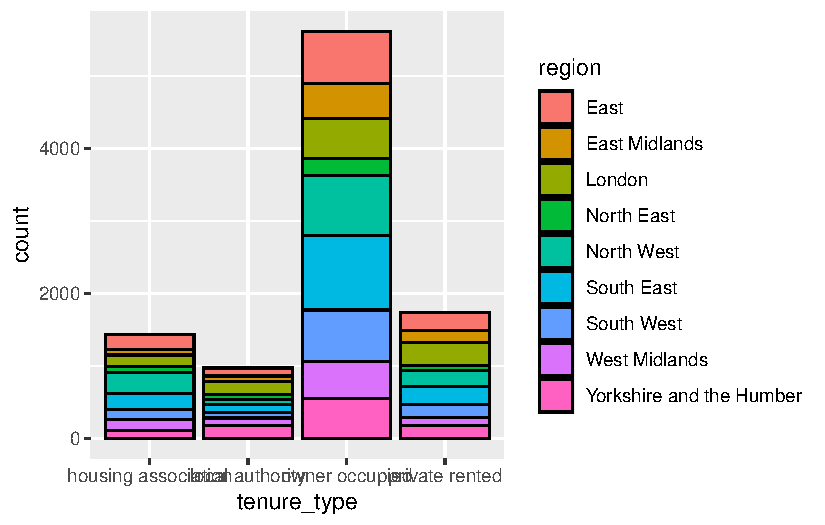
\includegraphics{visualisation_files/figure-pdf/stacked bar chart tenure-1.pdf}

\begin{tcolorbox}[enhanced jigsaw, bottomrule=.15mm, left=2mm, leftrule=.75mm, bottomtitle=1mm, coltitle=black, colbacktitle=quarto-callout-tip-color!10!white, toptitle=1mm, arc=.35mm, breakable, title=\textcolor{quarto-callout-tip-color}{\faLightbulb}\hspace{0.5em}{Style tip}, rightrule=.15mm, toprule=.15mm, opacityback=0, opacitybacktitle=0.6, titlerule=0mm, colback=white, colframe=quarto-callout-tip-color-frame]

R contains a list of 657 pre-programmed colours that can be used to
create palettes (run \texttt{colours()} in the console for a full list).
Hexadecimal codes can also be included instead in the form
\texttt{\#rrggbb} (where rr (red), gg (green), and bb (blue) are numbers
between 00 and 99 giving the level of intensity of each colour).

\end{tcolorbox}

Each geom has different arguments that can be customised to adapt
visualisations. For example, \texttt{geom\_bar} has the
\texttt{position} argument which controls how additional groups are
displayed. By default, this argument is set to \texttt{"stack"} which
created a stacked bar chart as we saw in the last example. An
alternative would be to set this to \texttt{position\ =\ "dodge"} which
creates a \textbf{side-by-side bar chart}. Here, the tenure type bars
are separated into smaller bars per region, but are displayed next to
one another, rather than on top of each other:

\begin{Shaded}
\begin{Highlighting}[]
\FunctionTok{ggplot}\NormalTok{(}\AttributeTok{data =}\NormalTok{ ehs\_tidy) }\SpecialCharTok{+} 
  \CommentTok{\# Define the x axis and fill inside aes}
  \FunctionTok{geom\_bar}\NormalTok{(}\FunctionTok{aes}\NormalTok{(}\AttributeTok{x =}\NormalTok{ tenure\_type, }\AttributeTok{fill =}\NormalTok{ region),}
           \CommentTok{\# Manually define colour outside aes}
           \AttributeTok{colour =} \StringTok{"black"}\NormalTok{,}
           \CommentTok{\# Show bars side{-}by{-}side instead of stacked}
           \AttributeTok{position =} \StringTok{"dodge"}\NormalTok{)}
\end{Highlighting}
\end{Shaded}

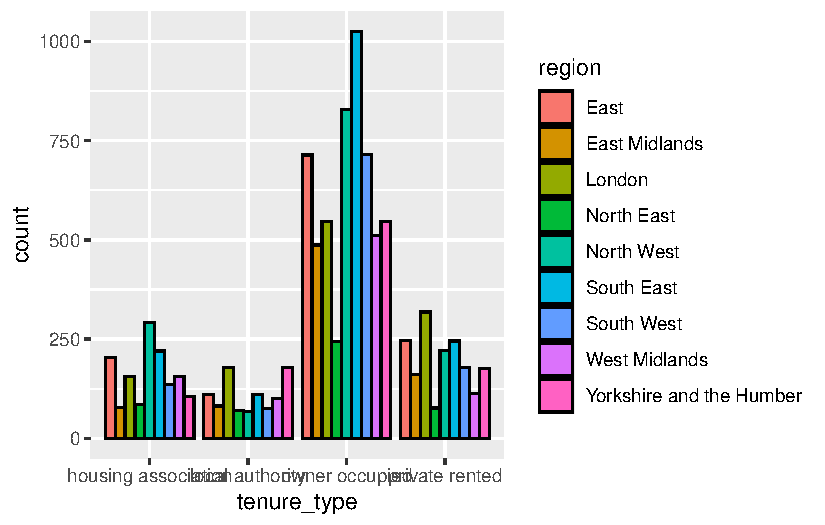
\includegraphics{visualisation_files/figure-pdf/side-by-side bar chart tenure-1.pdf}

For a more comprehensive list of the options available for the geom you
are interested in, check the helpfile (e.g.~\texttt{?geom\_bar}).

\begin{tcolorbox}[enhanced jigsaw, bottomrule=.15mm, left=2mm, leftrule=.75mm, bottomtitle=1mm, coltitle=black, colbacktitle=quarto-callout-warning-color!10!white, toptitle=1mm, arc=.35mm, breakable, title=\textcolor{quarto-callout-warning-color}{\faExclamationTriangle}\hspace{0.5em}{Warning}, rightrule=.15mm, toprule=.15mm, opacityback=0, opacitybacktitle=0.6, titlerule=0mm, colback=white, colframe=quarto-callout-warning-color-frame]

Although it may be tempting to add many variables to the same
visualisation, be sure that you are not overcomplicating the graph and
losing important messages. It is better to have multiple clear (but
simpler) visualisations than fewer confusing ones.

\end{tcolorbox}

\section{Exercise 8}\label{exercise-8}

Choose an appropriate visualisation to investigate the change in
employment rate between 2008 and 2024. Generate this visualisation and
comment on your findings.

\section{Scale functions}\label{scale-functions}

Scale functions allow us to customise aesthetics defined in geom
objects, such as colours and axes labels. They take the form
\texttt{scale\_\textquotesingle{}aesthetic\ to\ customise\textquotesingle{}\_\textquotesingle{}scale\ of\ variable’}.

\subsection{Customising axes}\label{customising-axes}

Scale functions can be used to customise axis titles, limits, breaks,
and labels. The choice of \texttt{scale} function is determined by the
type of variable displayed on the axis.

For example, if we wanted to customise the x axis of the line graph
generated in the previous exercise, showing the employment rate over
time, we would use the \texttt{scale\_x\_continuous} function. Arguments
to customise the x or y axes include:

\begin{itemize}
\tightlist
\item
  \texttt{name\ =} to change the axis title
\item
  \texttt{limits\ =\ c(...)} sets the axis limits
\item
  \texttt{breaks\ =\ c(...)} defines tick marks
\item
  \texttt{labels\ =\ c(...)} attaches labels to break values
\item
  \texttt{trans\ =} transforms the scale that the axis is shown on.
\end{itemize}

In this example, we can add labels to the x axis that shows which year
the time variable represents, making it easier to interpret:

\begin{Shaded}
\begin{Highlighting}[]
\FunctionTok{ggplot}\NormalTok{(}\AttributeTok{data =}\NormalTok{ obr\_data) }\SpecialCharTok{+}
  \FunctionTok{geom\_line}\NormalTok{(}\FunctionTok{aes}\NormalTok{(}\AttributeTok{x =}\NormalTok{ time, }\AttributeTok{y =}\NormalTok{ employment\_rate)) }\SpecialCharTok{+}
  \CommentTok{\# Add axis title}
  \FunctionTok{scale\_x\_continuous}\NormalTok{(}\AttributeTok{name =} \StringTok{"Year"}\NormalTok{, }
                     \CommentTok{\# Add breaks for each year}
                     \AttributeTok{breaks =} \FunctionTok{seq}\NormalTok{(}\DecValTok{1}\NormalTok{, }\DecValTok{65}\NormalTok{, }\AttributeTok{by =} \DecValTok{4}\NormalTok{),}
                     \CommentTok{\# Add labels to breaks}
                     \AttributeTok{labels =} \DecValTok{2008}\SpecialCharTok{:}\DecValTok{2024}\NormalTok{)}
\end{Highlighting}
\end{Shaded}

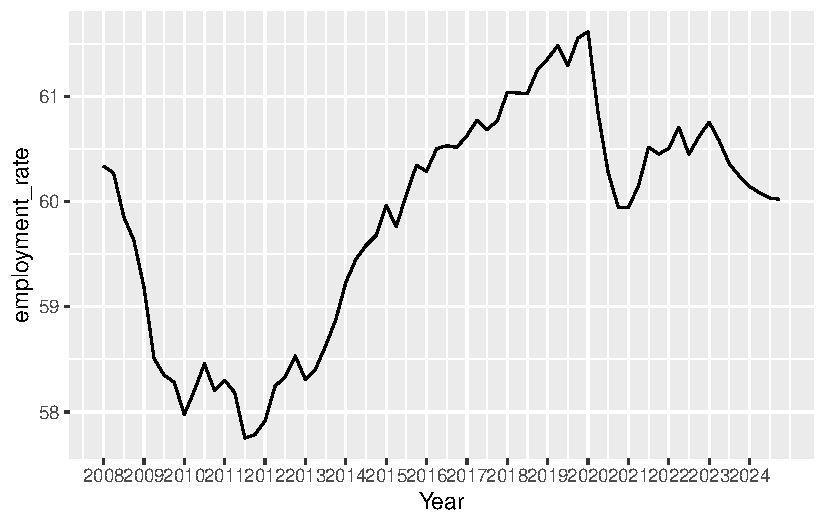
\includegraphics{visualisation_files/figure-pdf/line graph-1.pdf}

\subsection{Customising colour scales}\label{customising-colour-scales}

There are a wide range of options for customising the colour aesthetics
of geoms. These include pre-defined colour palettes, such as
\texttt{scale\_colour\_viridis\_c} for continuous variables, or
\texttt{scale\_colour\_viridis\_d} for discrete or categorical
variables. Viridis colour palettes are designed to be colourblind
friendly and print well in grey scale. There are also many R packages
containing colour palettes for different scenarios.

Colour palettes can be created manually for categorical variables using
the \texttt{scale\_colour\_manual} function. Here, the argument
\texttt{values} allows us to specify a colour per category.

Where a colour palette will be used across multiple plots, defining this
list of colours as a vector and then entering this into
\texttt{scale\_fill\_manual} will reduce repetition. For example, where
region is used to group across multiple plots, it will be useful to
create a region colour palette:

\begin{Shaded}
\begin{Highlighting}[]
\NormalTok{region\_palette }\OtherTok{\textless{}{-}} \FunctionTok{c}\NormalTok{(}\StringTok{"aquamarine2"}\NormalTok{, }\StringTok{"blue"}\NormalTok{, }\StringTok{"chartreuse2"}\NormalTok{, }\StringTok{"coral"}\NormalTok{, }\StringTok{"orchid"}\NormalTok{,}
                    \StringTok{"firebrick"}\NormalTok{, }\StringTok{"gold3"}\NormalTok{, }\StringTok{"violetred"}\NormalTok{, }\StringTok{"grey50"}\NormalTok{)}

\FunctionTok{ggplot}\NormalTok{(}\AttributeTok{data =}\NormalTok{ ehs\_tidy) }\SpecialCharTok{+} 
  \CommentTok{\# Define the x axis and fill inside aes}
  \FunctionTok{geom\_bar}\NormalTok{(}\FunctionTok{aes}\NormalTok{(}\AttributeTok{x =}\NormalTok{ tenure\_type, }\AttributeTok{fill =}\NormalTok{ region),}
           \CommentTok{\# Manually define colour outside aes}
           \AttributeTok{colour =} \StringTok{"black"}\NormalTok{,}
           \CommentTok{\# Show bars side{-}by{-}side instead of stacked}
           \AttributeTok{position =} \StringTok{"dodge"}\NormalTok{) }\SpecialCharTok{+}
  \CommentTok{\# Change legend title and add colour values}
  \FunctionTok{scale\_fill\_manual}\NormalTok{(}\AttributeTok{name =} \StringTok{"Region"}\NormalTok{, }\AttributeTok{values =}\NormalTok{ region\_palette)}
\end{Highlighting}
\end{Shaded}

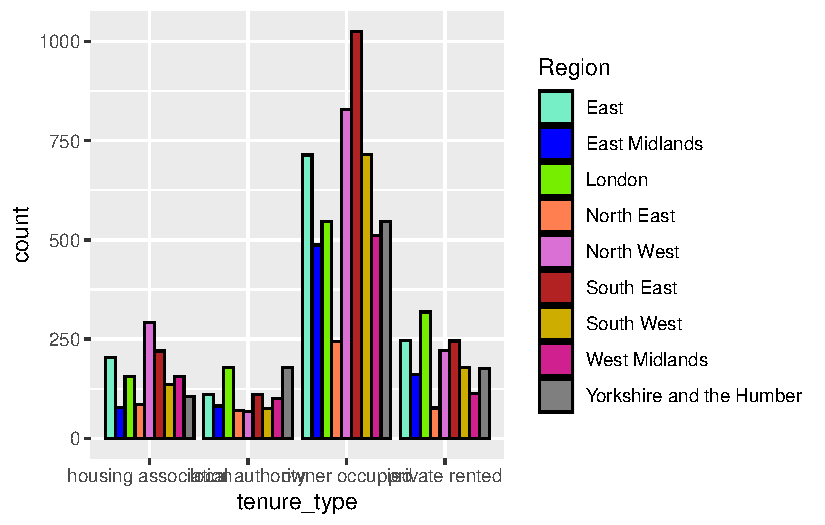
\includegraphics{visualisation_files/figure-pdf/region colour palette-1.pdf}

Palettes can also be created using gradients with the
\texttt{scale\_colour\_gradient} function, that specifies a two colour
gradient from low to high, \texttt{scale\_colour\_gradient2} that
creates a diverging gradient using low, medium, and high colours, and
\texttt{scale\_colour\_gradientn} that creates an n-colour gradient.

\section{Other labelling functions}\label{other-labelling-functions}

Although axis and legend labels can be updated within scale functions,
the \texttt{labs} function exist as an alternative. This function also
allows us to add titles and subtitles to visualisations:

\begin{Shaded}
\begin{Highlighting}[]
\FunctionTok{labs}\NormalTok{(}\AttributeTok{x =}\NormalTok{ “x}\SpecialCharTok{{-}}\NormalTok{axis name”, }\AttributeTok{y =}\NormalTok{ “y}\SpecialCharTok{{-}}\NormalTok{axis name”,}
    \AttributeTok{colour =}\NormalTok{ “Grouping variable name”, }\AttributeTok{title =}\NormalTok{ “Main title”,}
    \AttributeTok{subtitle =}\NormalTok{ “Subtitle”, }\AttributeTok{caption =}\NormalTok{ “Footnote”)}
\end{Highlighting}
\end{Shaded}

The \texttt{annotate} function allows us to add text and other objects
to a ggplot object. For example:

\begin{Shaded}
\begin{Highlighting}[]
\FunctionTok{annotate}\NormalTok{(“text”, }\AttributeTok{x =} \DecValTok{50}\NormalTok{, }\AttributeTok{y =} \DecValTok{200}\NormalTok{, }\AttributeTok{label =}\NormalTok{ “Text label here”)}
\end{Highlighting}
\end{Shaded}

Adds ``Text label here'' to a plot at the coordinates (50, 200) on a
graph, and

\begin{Shaded}
\begin{Highlighting}[]
\FunctionTok{annotate}\NormalTok{(“rect”, }\AttributeTok{xmin =} \DecValTok{0}\NormalTok{, }\AttributeTok{xmax =} \DecValTok{10}\NormalTok{, }\AttributeTok{ymin =} \DecValTok{20}\NormalTok{, }\AttributeTok{ymax =} \DecValTok{50}\NormalTok{, }\AttributeTok{alpha =} \FloatTok{0.2}\NormalTok{)}
\end{Highlighting}
\end{Shaded}

adds a rectangle to the graph.

\section{Theme functions}\label{theme-functions}

The \texttt{theme} function modifies non-data components of the
visualisation. For example, the legend position, label fonts, the graph
background, and gridlines. There are many options that exist within the
\texttt{theme} function (use \texttt{?theme} to list them all).

\begin{tcolorbox}[enhanced jigsaw, bottomrule=.15mm, left=2mm, leftrule=.75mm, bottomtitle=1mm, coltitle=black, colbacktitle=quarto-callout-note-color!10!white, toptitle=1mm, arc=.35mm, breakable, title=\textcolor{quarto-callout-note-color}{\faInfo}\hspace{0.5em}{Note}, rightrule=.15mm, toprule=.15mm, opacityback=0, opacitybacktitle=0.6, titlerule=0mm, colback=white, colframe=quarto-callout-note-color-frame]

Many of the elements that can be customised within the \texttt{theme}
function require an \texttt{element} wrapper. This wrapper is determined
by the type of object we are customising (e.g.~\texttt{element\_text}
when customising text, \texttt{element\_rect} when customising a
background, \texttt{element\_blank} to remove something). Check
\texttt{?theme} for more information.

\end{tcolorbox}

One of the most common theme options is \texttt{legend.position} which
can be used to move the legend to the top or bottom of the graph space
(\texttt{legend.position\ =\ “top”} or
\texttt{legend.position\ =\ “bottom”}) or remove the legend completely
(\texttt{legend.position\ =\ “none”}).

\texttt{ggplot} also contains a number of pre-defined themes which
change non-data elements of the plot to a programmed default. For
example \texttt{theme\_void} removes all gridlines and axes,
\texttt{theme\_light} changes the graph background white and the
gridlines and axes light grey:

\begin{Shaded}
\begin{Highlighting}[]
\FunctionTok{ggplot}\NormalTok{(}\AttributeTok{data =}\NormalTok{ ehs\_tidy) }\SpecialCharTok{+} 
  \CommentTok{\# Define the x axis and fill inside aes}
  \FunctionTok{geom\_bar}\NormalTok{(}\FunctionTok{aes}\NormalTok{(}\AttributeTok{x =}\NormalTok{ tenure\_type, }\AttributeTok{fill =}\NormalTok{ region),}
           \CommentTok{\# Manually define colour outside aes}
           \AttributeTok{colour =} \StringTok{"black"}\NormalTok{,}
           \CommentTok{\# Show bars side{-}by{-}side instead of stacked}
           \AttributeTok{position =} \StringTok{"dodge"}\NormalTok{) }\SpecialCharTok{+}
  \CommentTok{\# Change legend title and add colour values}
  \FunctionTok{scale\_fill\_manual}\NormalTok{(}\AttributeTok{name =} \StringTok{"Region"}\NormalTok{, }\AttributeTok{values =}\NormalTok{ region\_palette) }\SpecialCharTok{+} 
  \CommentTok{\# Remove gridlines and axes (not recommended!!)}
  \FunctionTok{theme\_void}\NormalTok{()}
\end{Highlighting}
\end{Shaded}

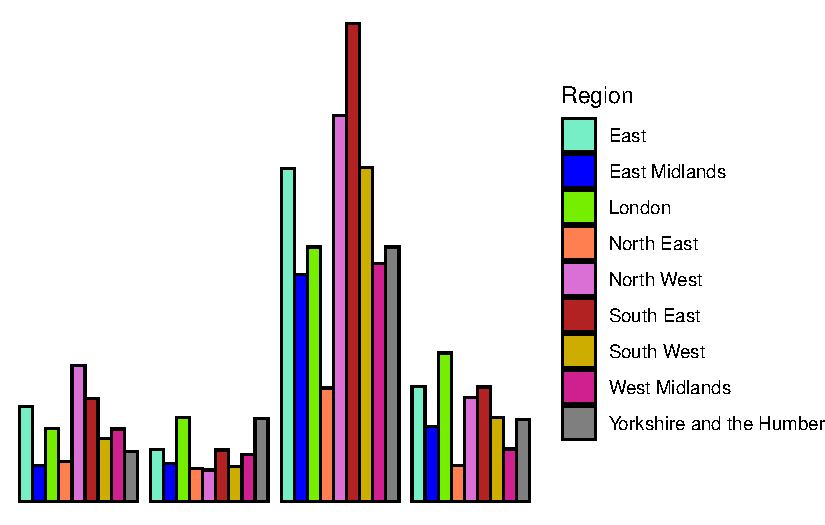
\includegraphics{visualisation_files/figure-pdf/side by side bar theme_light-1.pdf}

One benefit of using themes is that all visualisations will be
consistent in terms of colour scheme, font size and gridlines. Although
there are pre-built themes, we are able to create our own and save them
as functions. These can then be used in place of R's themes.

\subsection{Creating functions}\label{creating-functions}

To create our own function in R, we first give it a name and attach
\texttt{function()} followed by curly brackets \texttt{\{\}}, with the
function defined inside those brackets.

For example, to create our own theme function, called
\texttt{theme\_dluch}, which sets the title font size to 15, the axis
titles to size 12, the axis ticks to size 10, moves the legend to the
bottom of the graph, and changes the background colours, we use the
following:

\begin{Shaded}
\begin{Highlighting}[]
\NormalTok{theme\_dluch }\OtherTok{\textless{}{-}} \ControlFlowTok{function}\NormalTok{() \{}
  \CommentTok{\# Change plot title size}
  \FunctionTok{theme}\NormalTok{(}\AttributeTok{plot.title =} \FunctionTok{element\_text}\NormalTok{(}\AttributeTok{size =} \DecValTok{15}\NormalTok{),}
        \CommentTok{\# Change axis title size}
        \AttributeTok{axis.title =} \FunctionTok{element\_text}\NormalTok{(}\AttributeTok{size =} \DecValTok{12}\NormalTok{),}
        \CommentTok{\# Change axis text size}
        \AttributeTok{axis.text =} \FunctionTok{element\_text}\NormalTok{(}\AttributeTok{size =} \DecValTok{12}\NormalTok{),}
        \CommentTok{\# Move legend to bottom of graph}
        \AttributeTok{legend.position =} \StringTok{"bottom"}\NormalTok{,}
        \CommentTok{\# Change background}
        \AttributeTok{plot.background =} \FunctionTok{element\_rect}\NormalTok{(}\AttributeTok{fill =} \StringTok{"grey75"}\NormalTok{),}
        \CommentTok{\# Change graph area background}
        \AttributeTok{panel.background =} \FunctionTok{element\_rect}\NormalTok{(}\AttributeTok{fill =} \StringTok{"white"}\NormalTok{, }
                                        \AttributeTok{colour =} \StringTok{"black"}\NormalTok{))}
\NormalTok{\}}
\end{Highlighting}
\end{Shaded}

The function \texttt{theme\_dluch} will now appear in the Environment
window and can be added to \texttt{ggplot} objects:

\begin{Shaded}
\begin{Highlighting}[]
\FunctionTok{ggplot}\NormalTok{(}\AttributeTok{data =}\NormalTok{ ehs\_tidy) }\SpecialCharTok{+} 
  \CommentTok{\# Define the x axis and fill inside aes}
  \FunctionTok{geom\_bar}\NormalTok{(}\FunctionTok{aes}\NormalTok{(}\AttributeTok{x =}\NormalTok{ tenure\_type, }\AttributeTok{fill =}\NormalTok{ region),}
           \CommentTok{\# Manually define colour outside aes}
           \AttributeTok{colour =} \StringTok{"black"}\NormalTok{,}
           \CommentTok{\# Show bars side{-}by{-}side instead of stacked}
           \AttributeTok{position =} \StringTok{"dodge"}\NormalTok{) }\SpecialCharTok{+}
  \CommentTok{\# Change legend title and add colour values}
  \FunctionTok{scale\_fill\_manual}\NormalTok{(}\AttributeTok{name =} \StringTok{"Region"}\NormalTok{, }\AttributeTok{values =}\NormalTok{ region\_palette) }\SpecialCharTok{+} 
  \FunctionTok{labs}\NormalTok{(}\AttributeTok{x =} \StringTok{"Tenure type"}\NormalTok{, }\AttributeTok{y =} \StringTok{"Count"}\NormalTok{) }\SpecialCharTok{+}
  \CommentTok{\# Remove gridlines and axes (not recommended!!)}
  \FunctionTok{theme\_dluch}\NormalTok{()}
\end{Highlighting}
\end{Shaded}

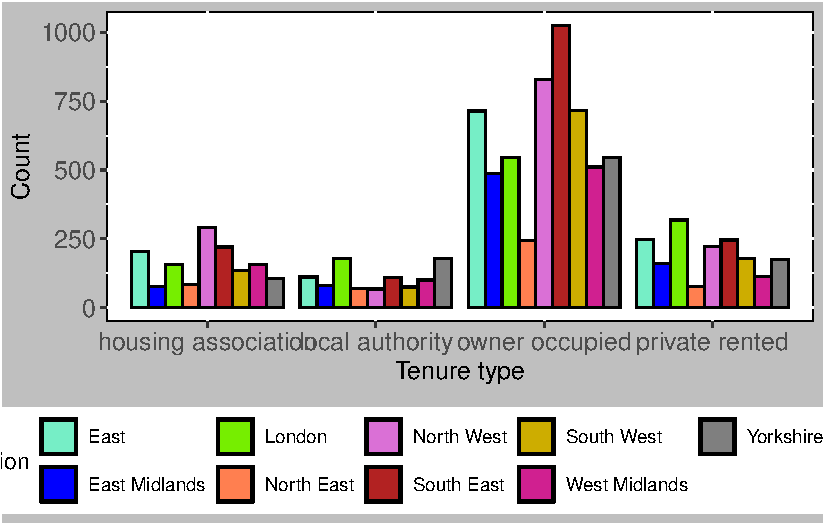
\includegraphics{visualisation_files/figure-pdf/side by side bar theme_dluch-1.pdf}

Creating a personalised theme ensures that visualisations are
consistent, whilst keeping code concise and reducing repetition.

\section{Facet functions}\label{facet-functions}

Faceting allows us to divide a plot into subplots based on some grouping
variable within the data. This allows us to show multiple variables in
the same visualisation without risking overloading the plot and losing
the intended message.

For example, we could compare the relationship between gross income and
tenure type (shown using a boxplot) between regions by faceting the
graph by region using the \texttt{facet\_wrap} function:

\begin{tcolorbox}[enhanced jigsaw, bottomrule=.15mm, left=2mm, leftrule=.75mm, bottomtitle=1mm, coltitle=black, colbacktitle=quarto-callout-warning-color!10!white, toptitle=1mm, arc=.35mm, breakable, title=\textcolor{quarto-callout-warning-color}{\faExclamationTriangle}\hspace{0.5em}{Warning}, rightrule=.15mm, toprule=.15mm, opacityback=0, opacitybacktitle=0.6, titlerule=0mm, colback=white, colframe=quarto-callout-warning-color-frame]

Remember that the value 100,000 actually represents anyone earning
£100,000 or more. To avoid skewing the data, we will remove these values
and investigate trends below this threshold.

\end{tcolorbox}

\begin{Shaded}
\begin{Highlighting}[]
\NormalTok{ehs\_tidy }\SpecialCharTok{\%\textgreater{}\%} 
  \CommentTok{\# Remove gross income \textgreater{}= £100,000}
  \FunctionTok{filter}\NormalTok{(gross\_income }\SpecialCharTok{!=} \DecValTok{100000}\NormalTok{) }\SpecialCharTok{\%\textgreater{}\%} 
  \CommentTok{\# Do not need to specify data, it is already passed through the pipes}
  \FunctionTok{ggplot}\NormalTok{() }\SpecialCharTok{+}
  \FunctionTok{geom\_boxplot}\NormalTok{(}\FunctionTok{aes}\NormalTok{(}\AttributeTok{x =}\NormalTok{ tenure\_type, }\AttributeTok{y =}\NormalTok{ gross\_income)) }\SpecialCharTok{+}
  \FunctionTok{labs}\NormalTok{(}\AttributeTok{x =} \StringTok{"Tenure type"}\NormalTok{, }\AttributeTok{y =} \StringTok{"Gross income (£)"}\NormalTok{) }\SpecialCharTok{+}
  \FunctionTok{facet\_wrap}\NormalTok{( }\SpecialCharTok{\textasciitilde{}}\NormalTok{ region) }\SpecialCharTok{+}
  \FunctionTok{theme\_dluch}\NormalTok{()}
\end{Highlighting}
\end{Shaded}

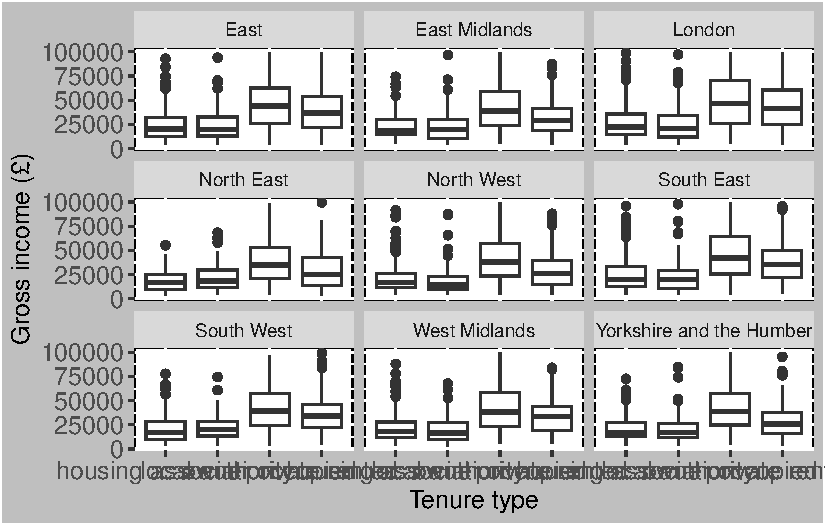
\includegraphics{visualisation_files/figure-pdf/boxplot income tenure region-1.pdf}

Facetting has made the tenure type labels unreadable. To overcome this,
we can `wrap' the long labels using the \texttt{label\_wrap\_gen}
function and setting an upper limit on the width of labels:

\begin{Shaded}
\begin{Highlighting}[]
\NormalTok{ehs\_tidy }\SpecialCharTok{\%\textgreater{}\%} 
  \CommentTok{\# Remove gross income \textgreater{}= £100,000}
  \FunctionTok{filter}\NormalTok{(gross\_income }\SpecialCharTok{!=} \DecValTok{100000}\NormalTok{) }\SpecialCharTok{\%\textgreater{}\%} 
  \CommentTok{\# Do not need to specify data, it is already passed through the pipes}
  \FunctionTok{ggplot}\NormalTok{() }\SpecialCharTok{+}
  \FunctionTok{geom\_boxplot}\NormalTok{(}\FunctionTok{aes}\NormalTok{(}\AttributeTok{x =}\NormalTok{ tenure\_type, }\AttributeTok{y =}\NormalTok{ gross\_income)) }\SpecialCharTok{+}
  \FunctionTok{scale\_x\_discrete}\NormalTok{(}\AttributeTok{labels =} \FunctionTok{label\_wrap\_gen}\NormalTok{(}\DecValTok{12}\NormalTok{)) }\SpecialCharTok{+}
  \FunctionTok{labs}\NormalTok{(}\AttributeTok{x =} \StringTok{"Tenure type"}\NormalTok{, }\AttributeTok{y =} \StringTok{"Gross income (£)"}\NormalTok{) }\SpecialCharTok{+}
  \FunctionTok{facet\_wrap}\NormalTok{( }\SpecialCharTok{\textasciitilde{}}\NormalTok{ region) }
\end{Highlighting}
\end{Shaded}

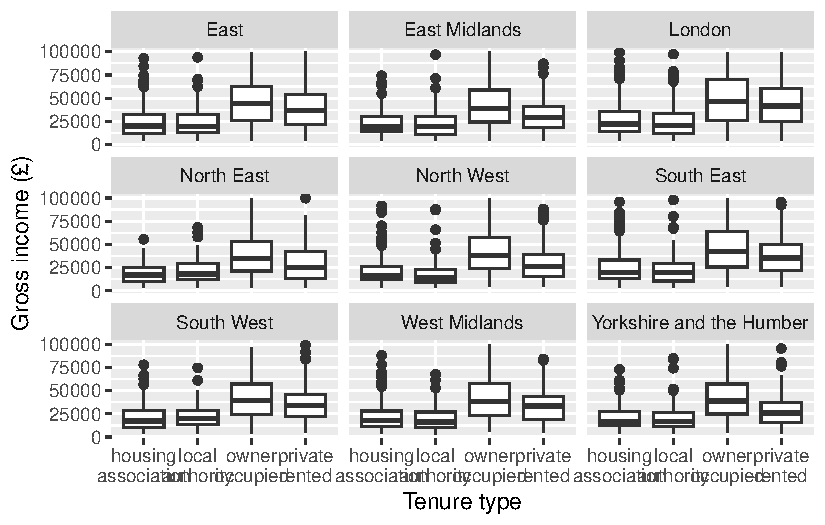
\includegraphics{visualisation_files/figure-pdf/boxplot income tenure region cleaner-1.pdf}

\section{Exercise 9}\label{exercise-9}

Use an appropriate visualisation to investigate the relationship between
house prices and wages between 2008 and now. Ensure that the variables
you choose are comparable and treat this as though the final product
will be exported into a report (make sure it is clear and looks good!).
Interpret your final graph.



\end{document}
